% Options for packages loaded elsewhere
\PassOptionsToPackage{unicode}{hyperref}
\PassOptionsToPackage{hyphens}{url}
\PassOptionsToPackage{dvipsnames,svgnames,x11names}{xcolor}
\documentclass[
  11pt,
  a4paper,
]{article}
\usepackage{xcolor}
\usepackage[margin=24mm]{geometry}
\usepackage{amsmath,amssymb}
\setcounter{secnumdepth}{-\maxdimen} % remove section numbering
\usepackage{iftex}
\ifPDFTeX
  \usepackage[T1]{fontenc}
  \usepackage[utf8]{inputenc}
  \usepackage{textcomp} % provide euro and other symbols
\else % if luatex or xetex
  \usepackage{unicode-math} % this also loads fontspec
  \defaultfontfeatures{Scale=MatchLowercase}
  \defaultfontfeatures[\rmfamily]{Ligatures=TeX,Scale=1}
\fi
\usepackage{lmodern}
\ifPDFTeX\else
  % xetex/luatex font selection
  \setmainfont[BoldFont=texgyrepagella-bold.otf,ItalicFont=texgyrepagella-italic.otf,BoldItalicFont=texgyrepagella-bolditalic.otf]{texgyrepagella-regular.otf}
  \setmonofont[BoldFont=lmmonolt10-bold.otf]{lmmono10-regular.otf}
  \setmathfont[]{texgyrepagella-math.otf}
\fi
% Use upquote if available, for straight quotes in verbatim environments
\IfFileExists{upquote.sty}{\usepackage{upquote}}{}
\IfFileExists{microtype.sty}{% use microtype if available
  \usepackage[]{microtype}
  \UseMicrotypeSet[protrusion]{basicmath} % disable protrusion for tt fonts
}{}
\makeatletter
\@ifundefined{KOMAClassName}{% if non-KOMA class
  \IfFileExists{parskip.sty}{%
    \usepackage{parskip}
  }{% else
    \setlength{\parindent}{0pt}
    \setlength{\parskip}{6pt plus 2pt minus 1pt}}
}{% if KOMA class
  \KOMAoptions{parskip=half}}
\makeatother
\usepackage{longtable,booktabs,array}
\usepackage{caption}
\captionsetup[table]{skip=6pt}
\newcounter{none} % for unnumbered tables
\usepackage{calc} % for calculating minipage widths
% Correct order of tables after \paragraph or \subparagraph
\usepackage{etoolbox}
\makeatletter
\patchcmd\longtable{\par}{\if@noskipsec\mbox{}\fi\par}{}{}
\makeatother
% Allow footnotes in longtable head/foot
\IfFileExists{footnotehyper.sty}{\usepackage{footnotehyper}}{\usepackage{footnote}}
\makesavenoteenv{longtable}
\usepackage{graphicx}
\makeatletter
\newsavebox\pandoc@box
\newcommand*\pandocbounded[1]{% scales image to fit in text height/width
  \sbox\pandoc@box{#1}%
  \Gscale@div\@tempa{\textheight}{\dimexpr\ht\pandoc@box+\dp\pandoc@box\relax}%
  \Gscale@div\@tempb{\linewidth}{\wd\pandoc@box}%
  \ifdim\@tempb\p@<\@tempa\p@\let\@tempa\@tempb\fi% select the smaller of both
  \ifdim\@tempa\p@<\p@\scalebox{\@tempa}{\usebox\pandoc@box}%
  \else\usebox{\pandoc@box}%
  \fi%
}
% Set default figure placement to htbp
\def\fps@figure{htbp}
\makeatother
\setlength{\emergencystretch}{3em} % prevent overfull lines
\providecommand{\tightlist}{%
  \setlength{\itemsep}{0pt}\setlength{\parskip}{0pt}}
\usepackage{mathtools}
\usepackage{graphicx}
\usepackage{needspace}
\usepackage{xurl}
\usepackage{etoolbox}
\usepackage{fancyhdr}
\usepackage{titlesec}
\setlength{\parindent}{0pt}
\setlength{\parskip}{5.5pt plus 1pt minus 1pt}
\setlength{\emergencystretch}{2em}
\clubpenalty=10000
\widowpenalty=10000
\displaywidowpenalty=10000
\raggedbottom
\pagestyle{fancy}
\fancyhf{}
\fancyfoot[C]{\small\thepage}
\renewcommand{\headrulewidth}{0pt}
\titleformat{\section}{\normalfont\Large\bfseries}{}{0pt}{}
\titlespacing*{\section}{0pt}{16pt plus 3pt minus 2pt}{7pt}
\pretocmd{\section}{\Needspace{6\baselineskip}}{}{}
\pretocmd{\subsection}{\Needspace{5\baselineskip}}{}{}
\makeatletter
\renewenvironment{figure}[1][]{\par\noindent\begin{minipage}{\linewidth}\def\@captype{figure}}{\end{minipage}\par\medskip}
\def\@maketitle{\newpage\null\begin{center}{\LARGE\bfseries\@title\par}\vskip .9em{\large\@author\par}\vskip .5em{\small\@date\par}\end{center}\vskip .4em}
\makeatother
\newsavebox{\papereqbox}
\newcommand{\paperdisplay}[2][]{\par\begingroup
\sbox{\papereqbox}{$\displaystyle #2$}
\typeout{PAPER-EQUATION-WIDTH: \the\wd\papereqbox; available \the\linewidth; tag #1}
\begin{equation*}\ifdim\wd\papereqbox>.93\linewidth
\resizebox{.93\linewidth}{!}{\usebox{\papereqbox}}\else\usebox{\papereqbox}\fi
\ifstrempty{#1}{}{\tag{#1}}\end{equation*}\endgroup\par}

\usepackage{bookmark}
\IfFileExists{xurl.sty}{\usepackage{xurl}}{} % add URL line breaks if available
\urlstyle{same}
% fallback for those not using the hyperref driver hyperxmp:
\makeatletter
\@ifundefined{xmpquote}{\newcommand{\xmpquote}[1]{#1}}{}
\makeatother
\hypersetup{
  pdftitle={The Tri-Octagon Z Manifold: Harmonic Macro Geometry{,} Chiral Deformation{,} and Diagnostic Dynamics},
  pdfauthor={Hilmir Frímann Halldórsson},
  colorlinks=true,
  linkcolor={MidnightBlue},
  filecolor={Maroon},
  citecolor={Blue},
  urlcolor={MidnightBlue},
  pdfcreator={LaTeX via pandoc}}

\title{The Tri-Octagon Z Manifold: Harmonic Macro Geometry, Chiral Deformation, and Diagnostic Dynamics}
\author{Hilmir Frímann Halldórsson}
\date{Paper E · Scientific review draft v0.1 · 23 September 2026}

\begin{document}
\maketitle

\section{1. Abstract}\label{abstract}

The historical Tri-Octagon program constructs an emergent readout from a three-component complex state and an independently advanced discrete clock. We reconstruct its scalar height, conical macro vector, quadratic chiral vector and direct blended trajectory, preserving the distinction between two historical scalar formulas. With amplitude frozen, the scalar is a third harmonic with three maxima and three minima. Its macro embedding lies exactly on a double cone; the six extrema form three vertical pairs with visiting order \(U_0,L_2,U_1,L_0,U_2,L_1\). The default twelve-sector clock misses those continuous extrema. The planar projection is a standard three-petal rose, with second- and fourth-harmonic Cartesian components. We prove the frozen-curve transformations and identify which descend to the sampled clock.

The chiral term is the oriented area \(\operatorname{Re}\Omega\times\operatorname{Im}\Omega\) in channel space. Its Gram determinant, transformation laws and sharp norm bound explain how the blend deforms the cone and can nearly cancel. We distinguish this direct trajectory from a scalar cylinder, a history-normalized torus and three channel-torus curves. The historical spike statistic combines displacement, inter-state phase, clock change and optional amplitude change; it is neither directional turning nor physical velocity. Two preserved spike datasets reproduce exactly in their saved Z, diagnostic and cubic-observable arrays when an omitted phase-synchronization setting is set to zero. The original execution environment is not thereby identified.

An exact one-step intensity budget separates cubic growth, graph coupling and the finite-step remainder. The underlying real-gradient increment does not guarantee a decrease of the potential under a finite update. The staged exponential envelope and the committed memory variant have different long-time readout behavior. The definitions and their geometry are closed within the inspected source scope. Spatial attachment to six author-recalled scaffold openings remains an explicit open interface. No physical energy, flux or conservation law is inferred.

\textbf{Preparation and status.} Author and design testimony: Hilmir Frímann Halldórsson. Source reconstruction, mathematical exposition, bounded checks and figures: Codex. GPT is the scientific lead named in the work order. The preceding historical reconstruction {[}R{]} is the accepted input to this manuscript; \textbf{scientific review of Paper E is pending GPT}. New derivations below are attributed to this preparation, not represented as recovered historical equations. The manuscript preserves the source formulas and does not modify either kernel or Papers A-D.

\section{2. Historical and source provenance}\label{historical-and-source-provenance}

\subsection{2.1 Evidence classes and the two cores}\label{evidence-classes-and-the-two-cores}

We use four distinct kinds of evidence. A \textbf{source definition} is an executable formula in the identified snapshot. An \textbf{exact derivation} is a consequence proved here under written hypotheses. A \textbf{numerical result} is an output of the specified finite computation, including its nonfinite entries. An \textbf{interpretation} relates those results to historical design testimony without treating the testimony as an equation. This separation is needed because similarly named visual objects use different maps, and two preserved core versions assign different meanings to the same scalar field.

The primary local source is the staged \texttt{kernel\_TO} tree, abbreviated \textbf{K}. Its \texttt{model\_core.py} implements the exponential-envelope scalar. The separate preserved committed-core snapshot, abbreviated \textbf{H}, implements a cubic-observable exponential moving average (EMA), added to an undamped harmonic. ``Committed'' identifies the provenance class of the preserved snapshot in {[}R{]}; it does not identify the exact original commit or runtime that produced either diagnostic dataset. Both snapshots are included byte-for-byte in this package. They are analyzed separately throughout.

The source-to-claim ledger gives precise function and line anchors. The following compact map organizes their roles; line numbering refers to the included unchanged snapshots.

{\def\LTcaptype{none} % do not increment counter
\begin{longtable}[]{@{}
  >{\raggedright\arraybackslash}p{(\linewidth - 2\tabcolsep) * \real{0.3500}}
  >{\raggedright\arraybackslash}p{(\linewidth - 2\tabcolsep) * \real{0.6500}}@{}}
\toprule\noalign{}
\begin{minipage}[b]{\linewidth}\raggedright
Evidence
\end{minipage} & \begin{minipage}[b]{\linewidth}\raggedright
Operative role
\end{minipage} \\
\midrule\noalign{}
\endhead
\bottomrule\noalign{}
\endlastfoot
K \texttt{model\_core.py}, lines 133, 169, 246, 268 & Complex update; staged scalar and three vectors; master step; pre-step history \\
H \texttt{model\_core.py}, \texttt{update\_z} & EMA scalar, with the same macro/chiral/blend construction \\
K \texttt{geometry\_3d.py}, lines 4, 25, 60 & Scalar cylinder; history torus; direct stored-vector extraction \\
K \texttt{geometry\_embeddings.py}, lines 6, 12, 19 & Configurable versions of the scalar embeddings \\
K \texttt{toy\_3d\_triocta.py}, lines 283, 649, 685, 826 & Channel-torus map; Z display scale; component selection; trail callback \\
K \texttt{definitions.py}, lines 117, 263, 340 & Direction metric; full geometric metric; entropy variant \\
K \texttt{z\_spike\_diagnostic.py}, lines 29, 72, 94 & Run setup; event selection; CSV, window and plot export \\
K \texttt{diagnostics.py}; \texttt{analysis\_tools.py}; \texttt{chirality\_lab.py} & Other initializers, plotting/curvature helpers and exploratory chirality consumers \\
\end{longtable}
}

The reconstruction {[}R{]} contains the broader bounded source closure and its 63 computational checks. The present package preserves that report and machine-readable results. It does not repeat the historical corpus search. Paper B {[}B{]}, v0.1.2, supplies the accepted interpretation of the channel-area triple. Paper D {[}D{]}, v0.1.1, supplies the clarified reference-scaffold construction. Neither paper supplies a registration of Z coordinates to six gap anchors.

\subsection{2.2 What the recovered setting establishes}\label{what-the-recovered-setting-establishes}

Two saved series labelled subcritical and critical were retained with parameter summaries. The summaries omit the phase-synchronization strength. The current inspected K default is \(\lambda_{\mathrm{phase}}=0.001\). The earlier bounded investigation found that the same inspected source, with \(\lambda_{\mathrm{phase}}=0\), exactly reproduces both saved Z arrays and their full saved spike statistic. The present fixed replays also verify the saved cubic observable \(J\), including matching nonfinite locations.

This is strong evidence for an effective phase-off configuration compatible with the artifacts. It does not prove that the original author explicitly supplied that keyword, that the original source possessed the same phase routine, or that the runtime, operating system and commit were identical. A prior implementation without the phase operation could produce the same effective map. We therefore report recovered effective settings, not a recovered original execution environment. The summaries and CSVs remain unchanged.

\subsection{2.3 Reproducibility and attribution}\label{reproducibility-and-attribution}

New Paper E checks comprise 66 exact symbolic predicates and four fixed source-body replays for figure data: a baseline, the EMA counterpart, and the two saved configurations. The existing 23-run bounded parameter evidence in {[}R{]} is reused without another sweep. The new replay result file explicitly identifies itself as Codex re-execution evidence. A preserved verification log is likewise earlier deterministic re-execution output, not an original captured-run file. The package records hashes of inputs, figures, source snapshots, manuscript and PDF.

Standard mathematics is cited selectively. The rose terminology is checked against Erb {[}Erb{]}, specifically the odd-petal convention in Example 3(iv). The channel-area identity is the familiar Gram/Lagrange identity {[}VA{]}. The graph sign convention is compared with the positive Laplacian in Spielman {[}SG{]}. All model-specific identities used here are proved in the manuscript. No novelty is claimed for these standard constructions.

\section{3. State, definitions and update order}\label{state-definitions-and-update-order}

\subsection{3.1 The readout hierarchy}\label{the-readout-hierarchy}

Let \(\Omega=(\Omega_1,\Omega_2,\Omega_3)^T\in\mathbb C^3\) and write \(\Omega=x+iy\) with \(x,y\in\mathbb R^3\). Let \(q\) be the integer clock, \(N\) its number of sectors, and \(t\) the stored historical time. All formulas in exact derivations assume finite inputs unless a limiting or failure case is expressly discussed. Set

\paperdisplay[1]{\kappa=\|\Omega\|_2,\qquad \rho=\frac{\kappa}{1+\kappa},\qquad \theta=\frac{2\pi q}{N}.}

The staged scalar and vectors are

\paperdisplay[2]{\begin{aligned}
z&=\lambda_{vp}\rho\cos\bigl(3(\theta-\ell)\bigr)e^{-\gamma t},\qquad \ell=\theta_{\mathrm{lock}},\\
M&=Z_{\mathrm{macro}}=z(\cos\theta,\sin\theta,1)^T,\\
C&=Z_{\mathrm{chiral}}=
\bigl(\Im(\bar\Omega_2\Omega_3),\Im(\bar\Omega_3\Omega_1),\Im(\bar\Omega_1\Omega_2)\bigr)^T,\\
T&=Z_{\mathrm{total}}=Z_{\mathrm{vec}}=\alpha M+\beta C.
\end{aligned}}

The source defaults are \(N=12\), clock increment one, \(\lambda_{vp}=0.618\), \(\gamma=0.577\), \(\ell=0.244\) radians, \(\alpha=1\) and \(\beta=0.5\). The first constant is the literal decimal in the code; it is not silently replaced by an exact algebraic number. None of these coordinates or parameters carries a recovered physical calibration. The clock angle is not the mean phase of \(\Omega\).

The legacy name \texttt{Z\_vec} and the history key \texttt{Z\_total} store the same vector. They do not define an additional evolved variable. The initial dataclass fields for \(z,M,C,T\) are zero, even when a nonzero \(\Omega\) has been supplied. Equation (2) describes the recomputed readout after an update, not a constraint enforced by the constructor on row zero.

\subsection{3.2 The complex recurrence}\label{the-complex-recurrence}

For real \(\epsilon,g,k_i\), complex forcing \(\delta\), and componentwise multiplication \(\odot\), the pre-synchronization update is

\paperdisplay[3]{V=\Omega+\epsilon\Omega\odot(k-|\Omega|^2)+gL_3\Omega+\delta,
\qquad
L_3=\begin{pmatrix}-2&1&1\\1&-2&1\\1&1&-2\end{pmatrix}.}

If \(V_j=r_j e^{i\varphi_j}\), the separate simultaneous phase operation is

\paperdisplay[4]{\varphi'_j=\varphi_j+\lambda_{\mathrm{phase}}
\sum_{k=1}^3\sin\bigl(3(\varphi_k-\varphi_j)\bigr),
\qquad V'_j=r_j e^{i\varphi'_j}.}

It preserves each magnitude mathematically. The source treats the phase-off setting as a disabled operation. Optional complex Gaussian noise is added afterwards, before committing \(\Omega\). Its standard deviation is zero in the runs analyzed here. The model runner\textquotesingle s \texttt{seed} metadata does not itself seed the optional global noise generator. Our finite replays construct the initial state with the recorded NumPy generator seed and leave noise disabled.

\textbf{The historical \texttt{dt} does not multiply (3) or (4).} It increments \(t\) after the complex update and therefore changes the staged envelope at a given row number. The parameter named \texttt{eps} controls the on-site cubic increment; it is not interchangeable with \texttt{dt}. Decreasing \texttt{dt} alone is not a convergence refinement of the entire recurrence.

\subsection{3.3 Recording and dependency order}\label{recording-and-dependency-order}

Each loop first records the current state, then performs (3), phase synchronization, optional noise, commitment of \(\Omega\), advancement of \(q\), advancement of \(t\), recomputation of \(z,M,C,T\), and finally cycle/identity diagnostics. Figure 1 retains that order, grouping boxes only for legibility.

\begin{figure}
\centering
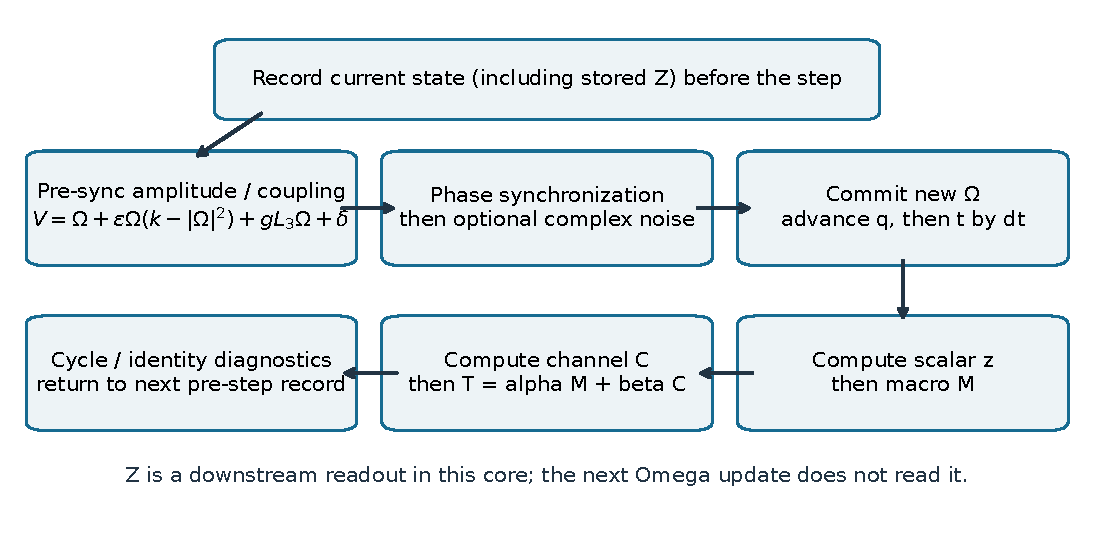
\includegraphics[width=0.95\linewidth,height=\textheight,keepaspectratio,alt={Exact historical dependency and recording order. The final instruction returns to the next pre-step record; it is not feedback from Z into the complex update.}]{figures/01_update_order.pdf}
\caption{Exact historical dependency and recording order. The final instruction returns to the next pre-step record; it is not feedback from Z into the complex update.}
\end{figure}

For \(n\) requested steps, stored row \(j\) is the state before update \(j\), for \(j=0,\ldots,n-1\). The state after update \(n-1\) remains available to the caller but is beyond the final recorded row. With default initialization, row zero has nonzero \(\Omega\) and zero Z. The first drawn segment therefore includes an initialization convention. It cannot be read as evidence of emission from a physical origin.

In this inspected core, the next complex update depends on \(\Omega\) and its update parameters, not on \(z,M,C,T\). The clock and Z coefficients are absent from (3)-(4). This is a source-scoped absence of feedback, not a claim about every consumer in the historical project. The bounded source closure {[}R{]} identifies a cloned-state option-volume probe, an external turning-triggered event consumer and a separate J-to-RSB parameter handoff. Such downstream uses do not alter the dependency of the retained recurrence analyzed here.

\section{4. The scalar Z harmonic}\label{the-scalar-z-harmonic}

\subsection{4.1 Continuous frozen-angle theorem}\label{continuous-frozen-angle-theorem}

Freeze \(\kappa,t,\lambda_{vp},\gamma\) and \(\ell\), and define

\paperdisplay[5]{A=\lambda_{vp}\rho e^{-\gamma t},\qquad f_\ell(\theta)=A\cos\bigl(3(\theta-\ell)\bigr).}

\textbf{Theorem 1 (six scalar extrema).} If \(A>0\), a full turn contains exactly three maxima at \(\ell+2\pi j/3\) and three minima at \(\ell+(2j+1)\pi/3\), \(j=0,1,2\), modulo \(2\pi\). Their values are \(A\) and \(-A\), respectively. Successive extrema alternate with angular separation \(\pi/3\). If \(A<0\), the locations remain critical and the maximum/minimum labels reverse. If \(A=0\), the function is constant and has no six isolated extrema.

\textbf{Proof.} Differentiating gives

\paperdisplay[6]{f'_\ell=-3A\sin\bigl(3(\theta-\ell)\bigr),\qquad
f''_\ell=-9A\cos\bigl(3(\theta-\ell)\bigr).}

For nonzero \(A\), critical angles are precisely \(\theta=\ell+k\pi/3\), with six distinct residues modulo \(2\pi\). At even \(k\), \(f=A\) and \(f''=-9A\); at odd \(k\), \(f=-A\) and \(f''=9A\). The second derivatives are nonzero, proving the classification and exhausting all critical points. Changing \(\ell\) translates this angular pattern. The zero-amplitude case follows directly from (5). \(\square\)

This is an angular theorem with frozen amplitude. Along a run, \(\kappa\) and \(t\) change, so \(A\) changes. Even if one chose a continuous interpolation, differentiating it would introduce the derivative of \(A\). The theorem does not assert fixed temporal maxima of that new interpolant. The source itself advances a discrete clock and does not supply this continuous interpolation.

\subsection{4.2 What the twelve-sector clock samples}\label{what-the-twelve-sector-clock-samples}

At \(\theta_q=\pi q/6\) and \(A\ne0\),

\paperdisplay[7]{\frac{z_q}{A}=\cos\left(\frac{\pi q}{2}-3\ell\right),\qquad
(z_q/A)_{q=0}^{11}=(c,s,-c,-s,c,s,-c,-s,c,s,-c,-s),}

where \(c=\cos(3\ell)\) and \(s=\sin(3\ell)\). The sequence follows from the four quarter-turn values of cosine, repeated because the scalar frequency is three. This is a sampled value pattern, not six exactly reached continuous extrema.

\textbf{Proposition 2 (exact-hit condition).} For nonzero \(A\), the twelve-sector grid hits any, and hence all six, continuous extrema if and only if \(\ell\in(\pi/6)\mathbb Z\), modulo equivalent angular periods.

\textbf{Proof.} An exact extremum requires \(\pi q/2-3\ell\in\pi\mathbb Z\). Dividing by three gives \(\ell=\pi q/6-m\pi/3\), an integer multiple of \(\pi/6\). Conversely, if \(\ell=r\pi/6\), sectors \(q=r+2m\) reach every successive extremum. The six remaining sectors are scalar zeros. \(\square\)

At \(\ell=0.244\), \(c\simeq0.7438391736\) and \(s\simeq0.6683586491\). Neither is one or zero, so the source samples have the sign pattern \(++--\) repeated three times and miss every continuous extremum. At \(\ell=\pi/12\), \(c=s=1/\sqrt2\), giving adjacent equal positive and negative heights. Those plateaus still do not hit the continuous maxima. The distinction matters when counting visual arms, clock states or proposed attachment sites.

\begin{figure}
\centering
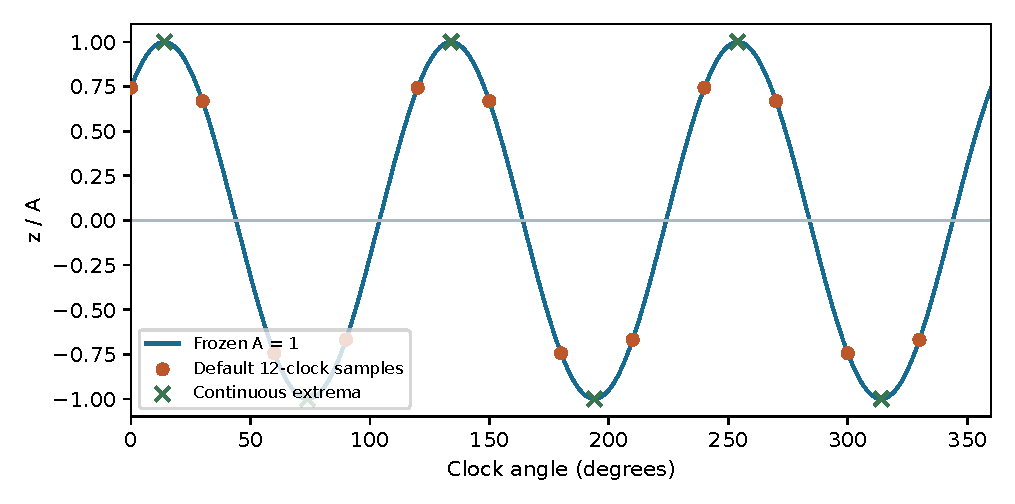
\includegraphics[width=0.94\linewidth,height=\textheight,keepaspectratio,alt={Frozen height with unit amplitude and default lock angle. Continuous extrema and twelve clock samples are shown separately; the clock samples do not attain the extrema.}]{figures/02_scalar_harmonic.pdf}
\caption{Frozen height with unit amplitude and default lock angle. Continuous extrema and twelve clock samples are shown separately; the clock samples do not attain the extrema.}
\end{figure}

\section{5. Macro Z as exact geometry}\label{macro-z-as-exact-geometry}

\subsection{5.1 Cone and norm}\label{cone-and-norm}

The macro map uses the scalar itself as both signed horizontal radius and height. It does not use \(\kappa\) as its horizontal radius. Define the quadratic form \(Q(X)=X_1^2+X_2^2-X_3^2\).

\textbf{Theorem 3 (macro cone).} For every finite scalar \(z\) and angle \(\theta\), the macro vector satisfies

\paperdisplay[8]{Q(M)=0,\qquad \|M\|_2=\sqrt2\,|z|.}

\textbf{Proof.} The first two squared coordinates sum to \(z^2(\cos^2\theta+\sin^2\theta)=z^2=M_3^2\). Adding the third squared coordinate yields \(2z^2\). Taking the nonnegative square root proves the norm identity. \(\square\)

This cone constraint holds even when the amplitude evolves, and also for the EMA scalar, because it uses only the definition of \(M\). By contrast, the detailed curve on the cone depends on which scalar law is used. At negative \(z\), the horizontal azimuth is \(\theta+\pi\) rather than \(\theta\). Neglecting this reversal produces an incorrect ordering of the lower extrema.

\subsection{5.2 Vertical pairing and visiting order}\label{vertical-pairing-and-visiting-order}

Assume frozen \(A>0\), and define \(a_j=\ell+2\pi j/3\). Let

\paperdisplay[9]{U_j=A(\cos a_j,\sin a_j,1)^T,\qquad
L_j=A(\cos a_j,\sin a_j,-1)^T.}

These are three vertical pairs, with horizontal coordinates at an equilateral triple. Their being vertical pairs is a statement in the direct macro coordinate system; no physical scaffold placement has been assumed.

\textbf{Theorem 4 (signed-extremum order).} Starting at \(\theta=\ell\) and increasing \(\theta\) through one full turn, the six scalar-extremum images under the macro map are visited in the order

\paperdisplay[10]{U_0\longrightarrow L_2\longrightarrow U_1\longrightarrow L_0
\longrightarrow U_2\longrightarrow L_1\longrightarrow U_0.}

\textbf{Proof.} At the even critical angle \(\ell+2j\pi/3\), the scalar is \(A\), giving \(U_j\). At the next critical angle \(\ell+(2j+1)\pi/3\), the scalar is \(-A\). Multiplication by this negative sign shifts the horizontal angle by \(\pi\), so the horizontal direction is \(\ell+(2j+4)\pi/3=a_{j+2}\) modulo \(2\pi\), while the height is \(-A\). Thus it is \(L_{j+2}\), with indices modulo three. Taking \(j=0,1,2\) gives (10). Equivalently, \(z(\theta+\pi)=-z(\theta)\) while the horizontal unit vector also reverses, which fixes the horizontal coordinates and reverses the height. \(\square\)

\begin{figure}
\centering
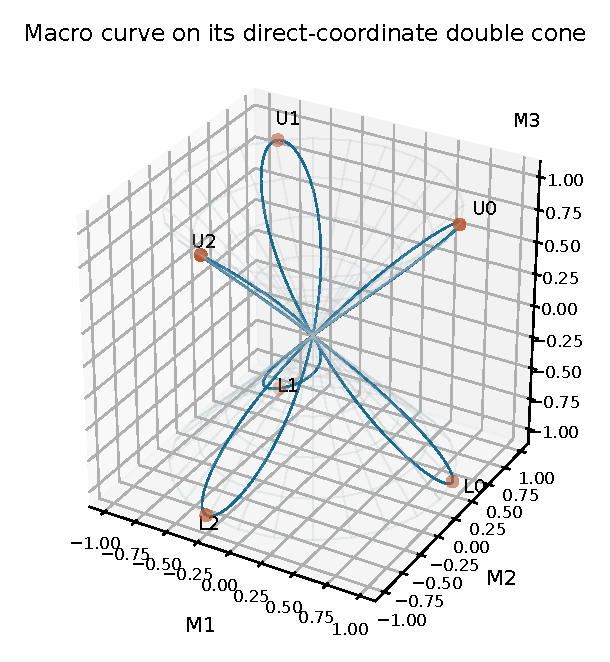
\includegraphics[width=0.82\linewidth,height=\textheight,keepaspectratio,alt={Frozen macro curve on its double cone. The marked extrema follow the proved visiting order. Labels identify mathematical points of the frozen curve, not recovered scaffold gaps.}]{figures/03_macro_cone.pdf}
\caption{Frozen macro curve on its double cone. The marked extrema follow the proved visiting order. Labels identify mathematical points of the frozen curve, not recovered scaffold gaps.}
\end{figure}

If \(A<0\), the entire frozen macro curve changes sign and the upper/lower naming must be adjusted. If \(A=0\), it collapses to the origin. The theorem is not a claim that an evolving default twelve-sector run passes through these six points: Proposition 2 excludes that at the default lock.

For the default sign pattern, the twelve nonzero frozen samples have six upper and six lower signed directions. Their horizontal azimuths are \(0^\circ,30^\circ,120^\circ,150^\circ,240^\circ,270^\circ\). Sectors \(q\) and \(q+6\) form vertical pairs only when their amplitudes agree. Along an evolving run, all sampled macro points remain on the cone, but their pair heights generally differ. The six horizontal azimuths of this sampled set must not be substituted for the six continuous extrema or for six spatial gaps.

\section{6. Planar harmonic decomposition}\label{planar-harmonic-decomposition}

\subsection{6.1 Cartesian harmonics and the rose}\label{cartesian-harmonics-and-the-rose}

Product-to-sum identities applied to (5) give

\paperdisplay[11]{\begin{aligned}
M_1(\theta)&=\frac A2\left[\cos(4\theta-3\ell)+\cos(2\theta-3\ell)\right],\\
M_2(\theta)&=\frac A2\left[\sin(4\theta-3\ell)-\sin(2\theta-3\ell)\right].
\end{aligned}}

For the first identity use \(2\cos u\cos v=\cos(u+v)+\cos(u-v)\) with \(u=3\theta-3\ell\) and \(v=\theta\). For the second use \(2\sin v\cos u=\sin(v+u)+\sin(v-u)\) and the oddness of sine. Thus a third-harmonic scalar does not mean that each Cartesian coordinate is a third harmonic: multiplication by the rotating unit vector shifts the frequencies to two and four.

The signed polar representation of the planar projection is \(r=A\cos(3(\theta-\ell))\). With \(u=\theta-\ell\), the curve is the standard three-petal rhodonea rotated by \(\ell\) and scaled by \(A\). Negative signed radius is interpreted in the usual polar manner by reversing the ray. Erb {[}Erb, Example 3(iv), p. 10{]} records the odd-frequency petal convention. We use that established term and make no novelty claim for rose geometry.

The planar projection has period \(\pi\): both its signed radius and horizontal direction change sign after half a turn. Consequently a \(2\pi\) parameter interval traces the planar rose twice. The three-dimensional macro curve is different: after half a turn the same horizontal point has opposite height. Its six passages through the origin occur where the scalar vanishes. The coincident branches at the origin mean that the image is not thereby a smooth embedded manifold. ``Z manifold'' is retained as the historical name of the construction, not used as an unproved topological classification.

\begin{figure}
\centering
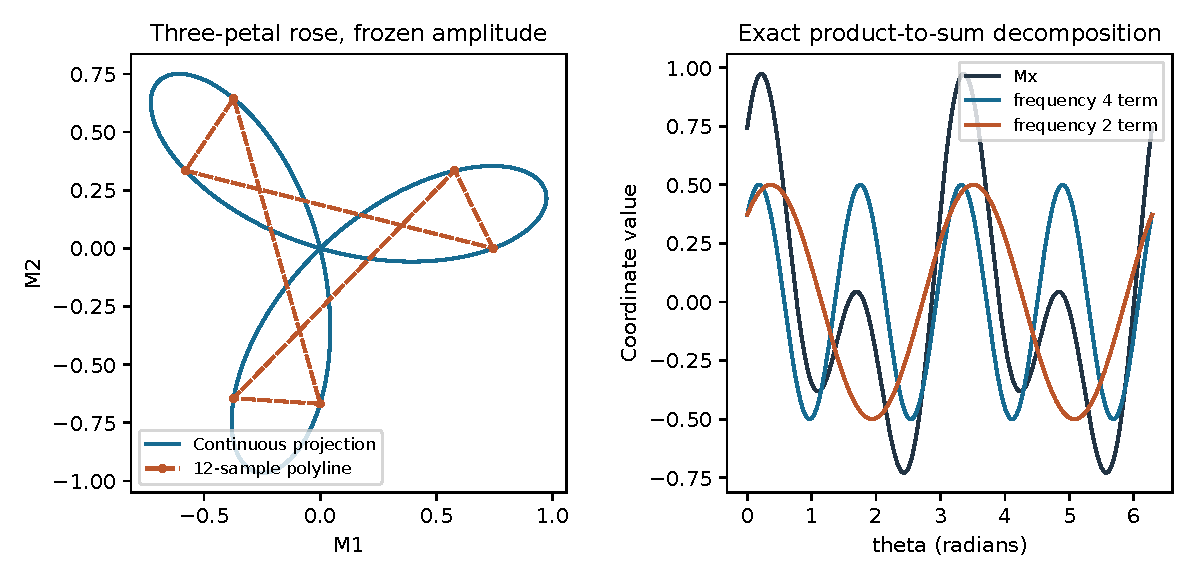
\includegraphics[width=0.98\linewidth,height=\textheight,keepaspectratio,alt={Planar rose and its twelve-sample polyline (left); the second- and fourth-harmonic summands of the first Cartesian coordinate (right). The second-coordinate decomposition is equation (11).}]{figures/04_rose_decomposition.pdf}
\caption{Planar rose and its twelve-sample polyline (left); the second- and fourth-harmonic summands of the first Cartesian coordinate (right). The second-coordinate decomposition is equation (11).}
\end{figure}

\subsection{6.2 From the analytic curve to the historical display}\label{from-the-analytic-curve-to-the-historical-display}

A plotted run connects finitely many sampled points by straight segments. Those segments need not lie on the analytic rose or on the double-cone surface; the endpoints obey the macro constraint. The endpoints are selected by the advancing clock while their radial factors change with \(\kappa\) and \(t\). Repeated visits to the same clock direction at different amplitudes can therefore accumulate several nearly parallel strands. Drawing the retained history at once superposes those strands, while a short moving window shows only a portion.

Four operations thus explain a multi-arm or star-like view without an additional force law: sampling the harmonic, changing its amplitude, joining samples by a polyline, and retaining multiple cycles of history. Adding \(\beta C\) then displaces each endpoint by a state-dependent channel-area vector. Fine visual splitting need not signal a new branch of an invariant manifold, and a crossing in a two-dimensional projection need not be a three-dimensional collision. The definitions support concrete geometry without those additional interpretations.

\section{7. Macro symmetry and its domains}\label{macro-symmetry-and-its-domains}

Let \(R_\delta\) be rotation by \(\delta\) about the third plotting axis, \(H=\operatorname{diag}(1,1,-1)\) and \(S=\operatorname{diag}(1,-1,1)\). Write \(M_\ell\) for the frozen-amplitude macro curve.

\textbf{Theorem 5 (frozen transformations).} At fixed \(A\), for all real angles,

\paperdisplay[12]{\begin{aligned}
M_\ell(\theta+2\pi/3)&=R_{2\pi/3}M_\ell(\theta),\\
M_\ell(\theta+\pi)&=H M_\ell(\theta),\\
M_\ell(-\theta)&=S M_{-\ell}(\theta),\\
M_\ell(2\ell-\theta)&=R_{2\ell}S M_\ell(\theta),\\
M_{\ell+\delta}(\theta)&=R_\delta M_\ell(\theta-\delta).
\end{aligned}}

\textbf{Proof.} A \(2\pi/3\) shift changes the harmonic argument by \(2\pi\), leaving \(z\) fixed while rotating its first two coordinate factors. A \(\pi\) shift reverses both \(z\) and the horizontal unit vector, proving the second line. Replacing \(\theta\) by \(-\theta\) uses the evenness of cosine in the scalar and reverses the sine coordinate, with lock \(-\ell\). The substitution \(2\ell-\theta\) leaves \(\cos(3(\theta-\ell))\) unchanged and reflects the horizontal unit vector in the line at azimuth \(\ell\). Finally, \(M_\ell(\theta-\delta)\) has the scalar of lock \(\ell+\delta\); multiplying by \(R_\delta\) restores the horizontal direction \(\theta\). These yield all five identities. \(\square\)

For the continuous frozen image, reparametrization runs over the entire circle, so these identities imply rotational and reflection symmetries of the image set. The third line alone is a relation between two lock choices; it is not a reflection symmetry at a generic fixed lock. The fourth line gives the appropriate fixed-lock reflection.

For the twelve-point frozen sample set, \(q\mapsto q+4\) and \(q\mapsto q+6\) are permutations. The first two transformations therefore descend to sampled points. The fixed-lock angular reflection maps the sampling grid into itself precisely when \(2\ell\) is an integer multiple of \(\pi/6\), equivalently \(\ell\in(\pi/12)\mathbb Z\). This is the grid condition for that inherited reflection; it is not an exhaustive classification of all accidental symmetries of degenerate sample images. At the default lock it fails. Arbitrary lock shifts rotate the continuous family but also change the clock\textquotesingle s sampling phase relative to that curve. A pure reindexing of the grid requires the angular shift to be a multiple of \(\pi/6\).

For an evolving trajectory, replacing \(q\) by \(q+4\) usually selects a different \(\kappa\), time and chiral term. Neither fixed \(A\) nor fixed \(C\) is then available. Thus exact symmetry of the frozen analytic image does not prove exact symmetry of a finite recorded path. Unequal on-site coefficients, initial conditions and phase evolution may further break visual symmetry of the total. The distinction is mathematical, not a plotting imperfection.

\section{8. Chiral Z in channel space}\label{chiral-z-in-channel-space}

\subsection{8.1 Oriented area and transformation laws}\label{oriented-area-and-transformation-laws}

Paper B {[}B{]} establishes the channel-space interpretation used here. The ordered channel coordinates, with their chosen orientation, determine the cross product. They are not a recovered ambient physical frame.

\textbf{Theorem 6 (channel area).} For \(\Omega=x+iy\),

\paperdisplay[13]{C=x\times y.}

Indeed \(\Im(\bar\Omega_j\Omega_k)=x_jy_k-y_jx_k\); listing the cyclic pairs \((2,3),(3,1),(1,2)\) gives the cross product. It is the oriented parallelogram-area triple of the real and imaginary channel vectors. It vanishes when those vectors are linearly dependent, which includes but is not restricted to real \(\Omega\).

For any complex \(c\) and any real common phase \(\chi\),

\paperdisplay[14]{C(e^{i\chi}\Omega)=C(\Omega),\qquad
C(\bar\Omega)=-C(\Omega),\qquad
C(c\Omega)=|c|^2 C(\Omega).}

\textbf{Proof.} A common phase rotates the ordered pair \((x,y)\) by a real two-dimensional rotation of determinant one. Bilinearity and antisymmetry therefore preserve \(x\times y\). Conjugation replaces \(y\) by \(-y\). Writing \(c=a+ib\) gives \(x'=ax-by\) and \(y'=bx+ay\), whose cross product is \((a^2+b^2)x\times y\). These arguments also cover \(c=0\). \(\square\)

Common-phase invariance is not invariance under arbitrary independent channel phases. Those phases change the pairwise imaginary products and are precisely part of the information carried by \(C\). Nor should this quadratic triple be confused with the cubic scalar

\paperdisplay[15]{J=\Im(\Omega_1\bar\Omega_2\Omega_3).}

The underlying cubic product acquires a factor \(e^{i\chi}\) under a common phase, so \(J\) is generally not common-phase invariant. It changes sign under conjugation, but it is not a component of \(C\) and does not universally determine the orientation or magnitude of the triple.

\subsection{8.2 Gram determinant and sharp bound}\label{gram-determinant-and-sharp-bound}

\textbf{Theorem 7 (area norm and equality case).} For finite \(\Omega\),

\paperdisplay[16]{\|C\|^2=\|x\|^2\|y\|^2-(x\cdot y)^2,
\qquad \|C\|\le \frac{\kappa^2}{2}.}

Equality in the bound holds if and only if \(\|x\|=\|y\|\) and \(x\cdot y=0\), including the zero state.

\textbf{Proof.} Expanding \(\sum_{i<j}(x_i y_j-x_j y_i)^2\) yields \(\sum_{i,j}x_i^2y_j^2-\sum_{i,j}x_i y_i x_j y_j\), proving the Gram determinant formula. Since \(\kappa^2=\|x\|^2+\|y\|^2\), subtracting gives the exact nonnegative slack

\paperdisplay[17]{\frac{\kappa^4}{4}-\|C\|^2
=\frac{(\|x\|^2-\|y\|^2)^2}{4}+(x\cdot y)^2.}

It vanishes exactly under the two stated conditions. Taking nonnegative square roots proves the bound. \(\square\)

For example, \(x=(a,0,0)\) and \(y=(0,a,0)\) attain it with \(C=(0,0,a^2)\) and \(\kappa^2=2a^2\). A state with large \(\kappa\) may instead have \(C=0\) if \(x\) and \(y\) are parallel. The bound controls possible area for a given state norm; it does not say all amplitude growth becomes chirality. This is standard area mathematics {[}VA{]} applied to the specific channel observable.

The staged scalar has an imposed exponential envelope. \textbf{The chiral term has no imposed decay envelope; it need not decay.} It may decay, persist or grow on a particular trajectory. No physical angular momentum, magnetic field or ambient axial-vector identification is made. Such interpretations would require a separate map, transformation law and calibration beyond the source.

\section{9. The blended Z construction}\label{the-blended-z-construction}

\subsection{9.1 Norm, alignment and cancellation}\label{norm-alignment-and-cancellation}

For real \(\alpha,\beta\), let \(m=\|M\|\) and \(c=\|C\|\). The Euclidean norm expansion is

\paperdisplay[18]{\|T\|^2=\alpha^2m^2+\beta^2c^2+2\alpha\beta M\cdot C.}

The cross term is positive for constructive weighted alignment, negative for destructive weighted alignment, and zero when the weighted vectors are perpendicular or one vanishes. If \(mc>0\), one may write it as \(2\alpha\beta mc\cos\psi\) with \(\psi\) the unweighted angle between \(M\) and \(C\). With negative weights, the sign of \(\cos\psi\) alone is insufficient to determine constructive blending.

The triangle and reverse-triangle inequalities give

\paperdisplay[19]{\bigl||\alpha|m-|\beta|c\bigr|\le\|T\|\le|\alpha|m+|\beta|c.}

\textbf{Proposition 8 (pointwise cancellation).} If \(\beta\ne0\), then \(T=0\) exactly when \(C=-\alpha M/\beta\). If both weighted vectors are nonzero, this requires their lengths to agree and their directions to oppose. If \(\beta=0\), cancellation means \(\alpha M=0\); if \(\alpha=0\) and \(\beta\ne0\), it means \(C=0\). With both weights zero the total vanishes identically.

The proposition is an algebraic characterization, not a claim that every selected pair \((M,C)\) is attained by one common source state or by an actual orbit. The common-state constraints in (1)-(2) must still hold. Figure 6 illustrates vector addition only; it is not a new dynamical trajectory or a synthesized boundary law.

\begin{figure}
\centering
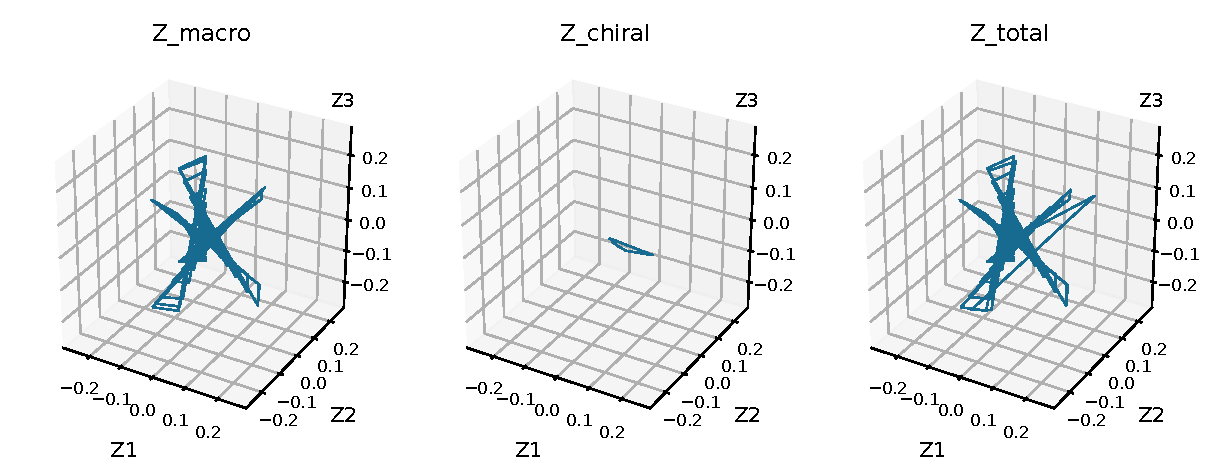
\includegraphics[width=1\linewidth,height=\textheight,keepaspectratio,alt={Baseline macro, chiral and total trajectories with a common raw coordinate scale. The source baseline has 300 stored rows. No viewer percentile normalization is applied.}]{figures/05_components.pdf}
\caption{Baseline macro, chiral and total trajectories with a common raw coordinate scale. The source baseline has 300 stored rows. No viewer percentile normalization is applied.}
\end{figure}

\begin{figure}
\centering
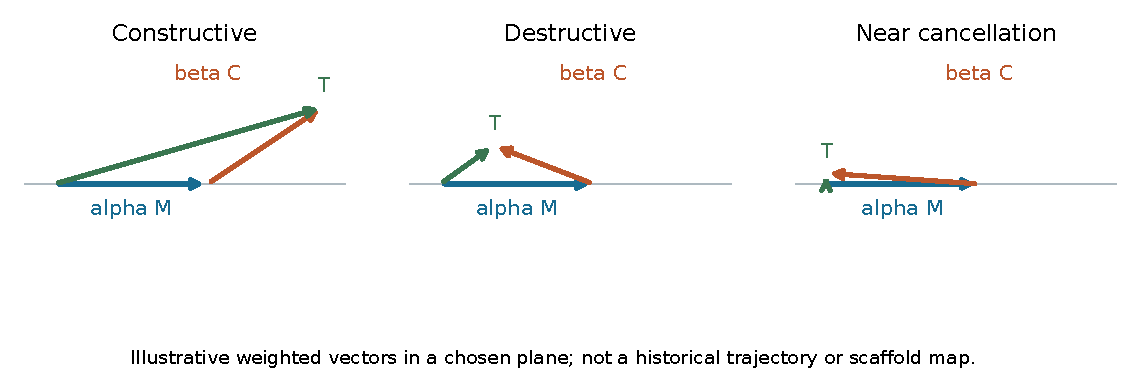
\includegraphics[width=1\linewidth,height=\textheight,keepaspectratio,alt={Weighted-vector alignment and cancellation geometry. The arrows absorb the coefficients. These algebraic examples illustrate vector addition rather than a fitted source trajectory.}]{figures/06_blend_alignment.pdf}
\caption{Weighted-vector alignment and cancellation geometry. The arrows absorb the coefficients. These algebraic examples illustrate vector addition rather than a fitted source trajectory.}
\end{figure}

\subsection{9.2 Leaving the cone and unstable directions}\label{leaving-the-cone-and-unstable-directions}

Because \(Q(M)=0\), direct expansion gives

\paperdisplay[20]{Q(T)=\beta^2Q(C)+2\alpha\beta(M_1C_1+M_2C_2-M_3C_3).}

Thus the total generally leaves the macro cone. Remaining on it at a point imposes the vanishing of the right side; it does not follow merely from the macro term dominating the visual shape. A point with total height of opposite sign to \(z\) is also possible, since \(T_3=\alpha z+\beta C_3\).

Near cancellation, direction is ill-conditioned even when the total displacement is small. For nonzero \(T\), let \(u=T/\|T\|\). Differentiation of normalization yields

\paperdisplay[21]{D\!\left(\frac{T}{\|T\|}\right)[h]=\frac{(I-uu^T)h}{\|T\|}.}

The tangent component of a perturbation is magnified by \(1/\|T\|\). For example, \(T_+=\eta e_2\) and \(T_-=-\eta e_2\) differ by only \(2\eta\) in norm but have opposite directions for every \(\eta>0\). At \(T=0\) there is no direction to normalize. Large directional change near the origin is therefore compatible with a small displacement statistic; it is not evidence for a large physical speed.

For \(\gamma t\ge0\) and finite \(\kappa\), \(|z|\le|\lambda_{vp}|\), hence \(\|M\|\le\sqrt2|\lambda_{vp}|\). Combining this with Theorem 7 bounds the total by \(\sqrt2|\alpha\lambda_{vp}|+|\beta|\kappa^2/2\). This is not a uniform bound over unbounded complex states. The saturation of \(\rho\) does not control the quadratic chiral term.

\subsection{9.3 Conjugation: a pointwise relation}\label{conjugation-a-pointwise-relation}

At fixed \(q,t\), parameters and staged formula, conjugating \(\Omega\) preserves \(\kappa\), \(z\) and \(M\), while reversing \(C\). Therefore

\paperdisplay[22]{T(\bar\Omega;q,t)=\alpha M-\beta C=2\alpha M-T(\Omega;q,t).}

This is point reflection about the state-dependent point \(\alpha M\) for the paired readouts. Since that point varies along a run, it is not generally a single rigid reflection of an entire trajectory. It also does not prove that conjugating one initial condition produces the paired state at every later step when external forcing or noise breaks conjugation covariance. The statement needs only the stated pointwise hypotheses.

In H, conjugation changes the cubic \(J\) and potentially the subsequent memory. The macro term then need not stay fixed, so (22) cannot be transferred to independently evolved EMA histories without an explicit condition that their scalar macros agree. Section 19 treats the memory formula separately.

\section{10. Alignment diagnostics and unresolved directions}\label{alignment-diagnostics-and-unresolved-directions}

The stored alignment histories are

\paperdisplay[23]{d_{TM}=u(T)\cdot u(M),\qquad d_{CM}=u(C)\cdot u(M),\qquad
d_{TC}=u(T)\cdot u(C).}

For finite vectors the historical helper defines \(u(v)=0\) if \(\|v\|<10^{-12}\) and \(u(v)=v/\|v\|\) otherwise. At exactly the threshold, it takes the normalized branch. When both inputs are resolved, each diagnostic is the cosine of the corresponding angle, bounded by \([-1,1]\) in exact arithmetic. The first expresses the total\textquotesingle s direction relative to the macro, the second compares the two ingredients, and the third expresses the total relative to the chiral contribution.

If either input is below the threshold, the stored dot is zero by implementation convention. This value does not prove geometric orthogonality: a tiny vector parallel to a large vector receives the same stored zero as an unresolved zero vector. The helper is not a general nonfinite sanitizer; NaNs are not converted into valid directions by the small-norm condition. Any interpretation of the diagnostic must first check finiteness and resolution.

The difference \(d_{TM}-d_{TC}\) can be used as an alignment preference score, but is not a decomposition of squared norm or an energy fraction. Equation (18), not the difference of these cosines, is the exact norm budget. In particular, positive alignment with both components can coexist with very different component lengths. A viewer that independently rescales the macro and chiral histories can conceal those length differences while leaving the within-history directions unchanged.

The direction-only spike routine uses another threshold, \(10^{-9}\), and returns unresolved values for unsuitable successive directions. That is a separate algorithm from the \(10^{-12}\) alignment helper. Keeping the thresholds and outputs distinct prevents an apparent zero or missing spike from being reinterpreted as an exact mathematical angle.

\section{11. Direct Z and the other historical displays}\label{direct-z-and-the-other-historical-displays}

\subsection{11.1 Four maps of different information}\label{four-maps-of-different-information}

The historical sources provide four coordinate constructions. They may receive related histories, but they are not interchangeable renderings of a single spatial point. To distinguish them, denote the scalar-cylinder map by \(F\), the history-torus map by \(G_{\mathcal H}\), the direct-vector map by \(T\), and the three channel curves by \(P_j\).

The scalar cylinder is

\paperdisplay[24]{F(\kappa,\theta,z)=(\kappa\cos\theta,\kappa\sin\theta,z).}

Its horizontal radius is the nonnegative state norm. In K \texttt{geometry\_3d.py}, the angle conversion is hardcoded to twelve sectors. The alternate configuration object in \texttt{geometry\_embeddings.py} exposes a sector count; it agrees for the historical default. Neither should silently inherit a different \(N\) selected elsewhere.

For a finite nonempty scalar history \(\mathcal H\), the torus map sets

\paperdisplay[25]{\begin{aligned}
H_z&=\max_{j\in\mathcal H}|z_j|+10^{-9},&
r&=r_{\max}\frac{\kappa}{1+\kappa},&
\chi&=\frac{\pi z}{2H_z},\\
G_{\mathcal H}(\kappa,\theta,z)
&=\bigl((R+r\cos\chi)\cos\theta,
(R+r\cos\chi)\sin\theta,r\sin\chi\bigr).
\end{aligned}}

The defaults are \(R=2\) and \(r_{\max}=1\). The regularizer makes \(|\chi|<\pi/2\) for finite histories, including their extrema. This map uses a whole-history maximum, not solely the current state. NaN-contaminated history maxima are not made meaningful by adding a regularizer.

The direct map simply takes the three stored columns of \(T\) in (2). It performs no torus construction, face selection or scaffold registration. Its default key can fall back to \texttt{Z\_vec}. The additional channel-torus curves instead use

\paperdisplay[26]{\begin{aligned}
\psi_j&=\frac{2\pi(j-1)}3,\qquad \eta_j=\arg\Omega_j,
\qquad r_j=0.6\bigl(1+0.4\log(1+|\Omega_j|)\bigr),\\
P_j&=\bigl((2+r_j\cos\eta_j)\cos\psi_j,
(2+r_j\cos\eta_j)\sin\psi_j,r_j\sin\eta_j\bigr).
\end{aligned}}

Here the major-ring channel azimuth is fixed for each channel; its phase moves around the local tube section and its magnitude changes that section\textquotesingle s radius. These three curves do not use the clock \(q\), scalar \(z\) or total \(T\). The title ``torus'' therefore covers two materially different display constructions even within the inspected source.

\subsection{11.2 Conditional inverse of the history torus}\label{conditional-inverse-of-the-history-torus}

\textbf{Proposition 9 (conditional torus inverse).} Suppose \(R>r_{\max}>0\), \(H_z>0\) is known and fixed, \(\kappa>0\) is finite, and the point is produced by (25) with \(|\chi|<\pi/2\). Then, modulo the angular period, its input is recovered by

\paperdisplay[27]{\begin{aligned}
s&=\sqrt{X^2+Y^2},\qquad u=s-R,\qquad
r=\sqrt{u^2+Z^2},\\
\theta&=\operatorname{atan2}(Y,X),\qquad
\chi=\operatorname{atan2}(Z,u),\\
\kappa&=\frac{r}{r_{\max}-r},\qquad
z=\frac{2H_z\chi}{\pi}.
\end{aligned}}

\textbf{Proof.} The major radius \(R+r\cos\chi\) is positive. Hence \(s=R+r\cos\chi\) and \((u,Z)=r(\cos\chi,\sin\chi)\). Since \(r>0\) and the angular branch is specified, the radial norm and two arguments recover \(r,\chi,\theta\). Inverting \(r=r_{\max}\kappa/(1+\kappa)\) gives the stated \(\kappa\), with \(0<r<r_{\max}\). The known normalization recovers \(z\). \(\square\)

\begin{figure}
\centering
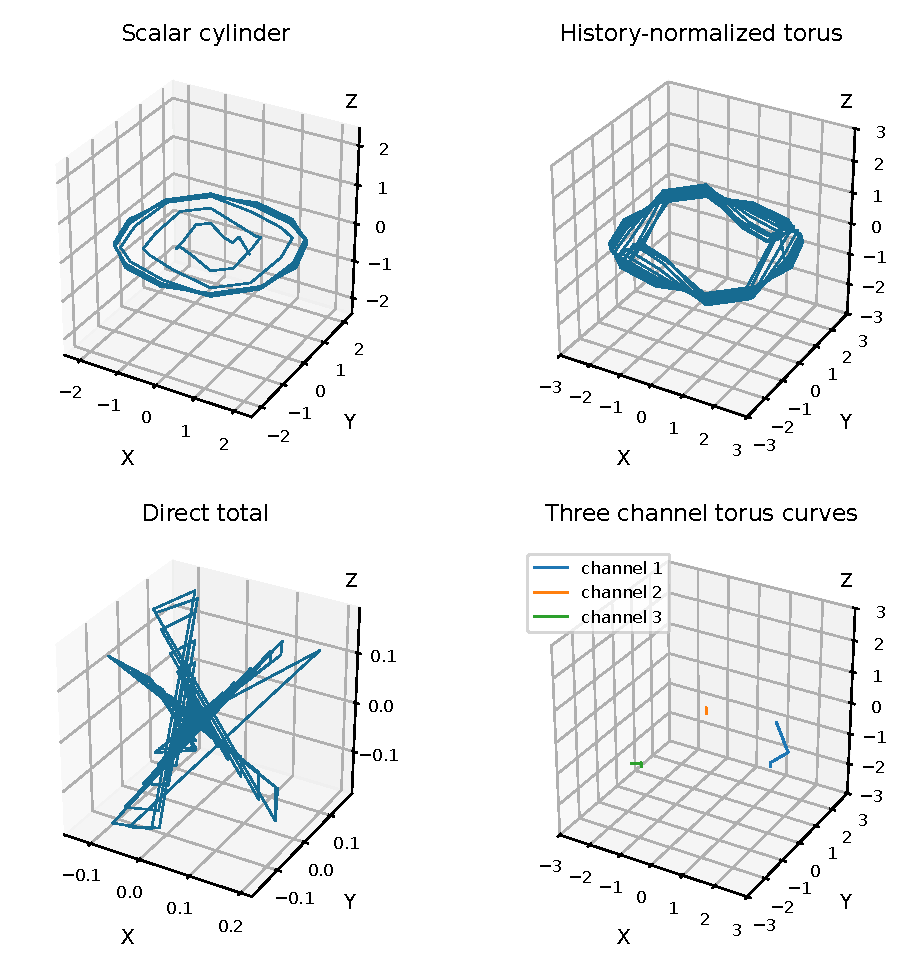
\includegraphics[width=0.93\linewidth,height=\textheight,keepaspectratio,alt={The four displays applied to the same baseline history. Axes have equal geometric units within each panel; numerical ranges differ between maps. The direct panel uses raw T.}]{figures/07_four_displays.pdf}
\caption{The four displays applied to the same baseline history. Axes have equal geometric units within each panel; numerical ranges differ between maps. The direct panel uses raw T.}
\end{figure}

The restriction \(\kappa>0\) excludes the degeneracy at \(r=0\), where the height information disappears. If \(H_z\) is unknown, the displayed minor angle gives only \(z/H_z\) and not \(z\). Appending a larger scalar excursion to a history changes \(H_z\) and therefore changes the displayed position of an earlier unchanged state. This directly disproves a universal pointwise coordinate change independent of history. Proposition 9 supplies a conditional inverse, not a claim of global equivalence to the direct Z map.

\subsection{11.3 A loss-of-information counterexample}\label{a-loss-of-information-counterexample}

Consider two recomputed staged states at the same \(q,t\) and parameters,

\paperdisplay[28]{\Omega^{(a)}=(1,1,1)^T,\qquad \Omega^{(b)}=(1,i,1)^T.
\qquad C^{(a)}=0,\quad C^{(b)}=(-1,0,1)^T.}

Both have \(\kappa=\sqrt3\), hence the same \(z\) and \(M\). They yield the same scalar-cylinder point and, if their scalar histories share the same normalization, the same history-torus point. Yet their totals differ by \(\beta(-1,0,1)^T\) whenever \(\beta\ne0\). This proves that \(T\) cannot in general be reconstructed from either scalar display. The lost relative-phase information is not restored by a camera rotation or a torus inverse. Conversely, knowing one total vector does not identify all complex state coordinates and clock history.

\section{12. Historical viewer scaling and selection}\label{historical-viewer-scaling-and-selection}

For the selected stored vector history \(Z_j\), the actual viewer forms norms, retains finite norms above \(10^{-12}\), and takes their 99th percentile. Let \(D_{99}\) denote that denominator, with fallback one when no suitable denominator exists. With frame minor radius \(r_{\mathrm{frame}}=0.6\), the displayed overlay is

\paperdisplay[29]{Z^{\mathrm{display}}_j=s_{\mathcal H,Z}Z_j,\qquad
s_{\mathcal H,Z}=\frac{0.85\,r_{\mathrm{frame}}}{D_{99}}.}

This is one positive scalar multiplication for the entire selected history. It preserves angles and relative lengths within that history and does not rotate the points. It does not preserve the raw scale between independently selected histories. A very small but nonzero chiral trajectory can be enlarged until it occupies much of the same frame as a much larger macro trajectory. The radio selections \texttt{Z\_total}, \texttt{Z\_macro} and \texttt{Z\_chiral} each recompute their own denominator; \texttt{off} hides the overlay.

The history dependence is retrospective. Adding a late excursion may alter the percentile and therefore rescale earlier points. Moreover, a percentile is not a maximum: values above the 99th percentile can extend beyond the nominal target size. Nonfinite points are excluded from the scale denominator but are not transformed into meaningful points by the scaling operation. A scientific comparison must state whether raw or normalized coordinates are being shown.

The trail-length callback shortens the three \(\Omega_j\) torus curves. It does not shorten the full Z overlay in the inspected implementation. A screenshot can therefore combine a short channel trail with a much longer retained Z history. The viewer\textquotesingle s alternative strong-change scalar uses the elevation-like quantity \(\operatorname{atan2}(T_3,\sqrt{T_1^2+T_2^2}+10^{-12})\), with fallback to the older scalar history; it is another display/diagnostic channel, not the definition of \(z\).

The UI variables named \texttt{gap\_top} and \texttt{gap\_bottom} place controls between panels. They are layout coordinates and provide no scaffold opening map. The separate viewer measurement-noise option perturbs certain scalar/observable histories after the complex and vector histories have been formed. It is not the optional complex noise in the core recurrence. Those source distinctions explain why different viewer choices cannot be used as interchangeable physical measurements.

All scientific component comparisons in this paper use raw coordinates. Each three-dimensional panel has equal spatial axis units; Figure 5 additionally uses one common range across all three components. Figure 7 compares different maps and therefore declares different numerical ranges. No figure uses (29) to disguise a relative magnitude difference.

\section{13. Spike-diagnostic mathematics}\label{spike-diagnostic-mathematics}

\subsection{13.1 The full statistic}\label{the-full-statistic}

Given successive stored rows, let the selected vector \(Z\) be total, macro or chiral. The default is total. The full \texttt{compute\_recursive\_velocity\_geom} statistic computes

\paperdisplay[30]{\begin{aligned}
d_Z(n)&=\|Z_{n+1}-Z_n\|_2,\\
d_\varphi(n)&=\left|\operatorname{wrap}_{[-\pi,\pi)}\arg
\left(\frac13\sum_{j=1}^3\Omega_{j,n+1}\bar\Omega_{j,n}\right)\right|,\\
d_q(n)&=\mathbf1\{q_{n+1}\ne q_n\},\qquad
d_\kappa(n)=|\kappa_{n+1}-\kappa_n|,\\
v_{\mathrm{rec}}(n)&=\sqrt{(w_Zd_Z)^2+(w_\varphi d_\varphi)^2+(w_qd_q)^2+(w_\kappa d_\kappa)^2}.
\end{aligned}}

There is no division by \texttt{dt} in this statistic. The weights combine an uncalibrated displacement with phase and clock terms; the result is not a physical velocity. The default weights are \((w_Z,w_\varphi,w_q,w_\kappa)=(1,1,0.5,0)\). The phase term is the argument of a mean complex inter-state product, not the mean of three wrapped channel phase increments. At a zero product the mathematical phase is undefined; the implementation uses NumPy\textquotesingle s angle convention. Missing optional histories can produce zero component arrays in this helper. Equation (30) describes the complete finite-history case.

\textbf{Proposition 10 (clock floor).} On each ordinary default clock transition, with finite arithmetic and all terms defined, \(v_{\mathrm{rec}}\ge0.5\).

\textbf{Proof.} The default twelve-sector increment changes \(q\) even when it wraps from eleven to zero, so \(d_q=1\). Its squared contribution is \(0.25\); every other squared term is nonnegative. \(\square\)

This floor would not apply to a clock increment that leaves the stored sector unchanged. It also does not repair overflow: for example, floating-point multiplication of a zero weight by an infinite component can produce NaN. The exact real-arithmetic identity and its finite numerical implementation have different domains near failure.

\subsection{13.2 Exact separating examples}\label{exact-separating-examples}

To compare definitions, first set phase and clock contributions to zero in the example histories. A radial change \(Z_n=(1,0,0)\) to \(Z_{n+1}=(10,0,0)\) has displacement nine and zero change of direction. A sign flip \(Z_n=\eta e_1\) to \(Z_{n+1}=-\eta e_1\) has displacement \(2\eta\) and direction angle \(\pi\). Taking \(\eta=10^{-8}\) keeps both directions above the direction routine\textquotesingle s threshold while making the displacement tiny. Finally, holding Z and \(\Omega\) fixed while changing only \(q\) gives \(v_{\mathrm{rec}}=0.5\) under the default weights and zero directional turning. These are exact separating inputs to the diagnostic definitions, not assertions that all three pairs follow one chosen orbit of (3).

The direction-only routine measures the angle between successive resolved vectors from the origin:

\paperdisplay[31]{a_n=\arccos\!\left(\operatorname{clip}\left(
\frac{Z_n\cdot Z_{n+1}}{\|Z_n\|\|Z_{n+1}\|},-1,1\right)\right).}

Polyline curvature instead compares consecutive segment directions, \(\Delta Z_{n-1}\) and \(\Delta Z_n\). It can be large where origin-based directions change little, and it is unresolved when a required segment vanishes. The entropy variant uses \(|H_{n+1}-H_n|\) for a spectral-entropy series. These are different functions of different inputs. Their shared historical name \texttt{v\_rec} does not identify one observable.

The separate \texttt{chirality\_lab.py} fits the cubic observable from Z and uses regularized finite-difference curvature and torsion. Those derivative estimates use the mean stored time step, unlike the full statistic (30). Its squared fitted geometric quantity is a diagnostic construction, not a recovered potential or conservation law. These exploratory consumers do not replace the source definitions of z, C or T.

\subsection{13.3 Thresholds, indexing and source limitations}\label{thresholds-indexing-and-source-limitations}

The spike exporter classifies finite full-statistic values by an absolute threshold, here \(0.8\), or by a selected high quantile, typically \(0.99\). A quantile threshold with an inclusive comparison may retain many tied values; it does not guarantee exactly one percent of events. Metric array entry \(n\) belongs to the transition ending at stored row \(n+1\). The CSV places a blank diagnostic at row zero and aligns later values with their endpoint rows. The source constructs displayed CSV times as row number times \texttt{dt}; accumulation in the core\textquotesingle s stored time can differ by floating-point roundoff.

Saved windows select \(\pm25\) rows around each event endpoint and clip indices to the available range. Overlapping windows and clipped repeated rows are therefore expected, not independent observations. The original plotting helper can show only the final 500 points with unequal automatic axis ranges. Such a plot is not a full-history, equal-scale geometric certificate.

The source closure also found technical limits that remain preserved: the picker reads a global diagnostic series, which its writer sets; one named coefficient-mode argument does not replace the actual default triplet; the viewer wrapper resolves a direction metric and has a problematic recursive fallback. Flat script imports also conflict with relative imports in the inspected core. The bounded harness loads inspected source bodies in an isolated package to test their numerical behavior without editing these originals. Successful numerical reproduction is not claimed to certify an unchanged end-to-end GUI launch.

\section{14. Mechanisms behind diagnostic spikes}\label{mechanisms-behind-diagnostic-spikes}

There are six mechanisms to keep separate. Large displacement directly increases \(d_Z\). Inter-state phase near \(\pi\) increases \(d_\varphi\), even without an unusually large displacement. Clock advancement contributes its fixed floor. Quadratic chiral growth can enlarge the total as \(\Omega\) grows. Near cancellation makes the normalized direction unstable but need not enlarge \(d_Z\). Finally, overflow and NaN terminate the finite numerical interpretation. Only the first four enter a finite full-statistic event directly through the specified components; near cancellation is particularly relevant to directional diagnostics.

Figure 8 uses the phase-off subcritical replay and chooses the largest finite statistic among transitions 1 through 63, excluding the initialization transition. It occurs at endpoint row 8, where \(d_Z\simeq0.97326494\), \(d_\varphi\simeq\pi\) and the weighted clock term is \(0.5\). Their quadratic combination gives \(v\simeq3.32668740\). The event is not explained by direction change alone. At endpoint row 501, \(d_Z\simeq0.01315546\) and the phase contribution is zero, leaving \(v\simeq0.50017304\). The later approach to the floor is a directly measured property of this run.

\begin{figure}
\centering
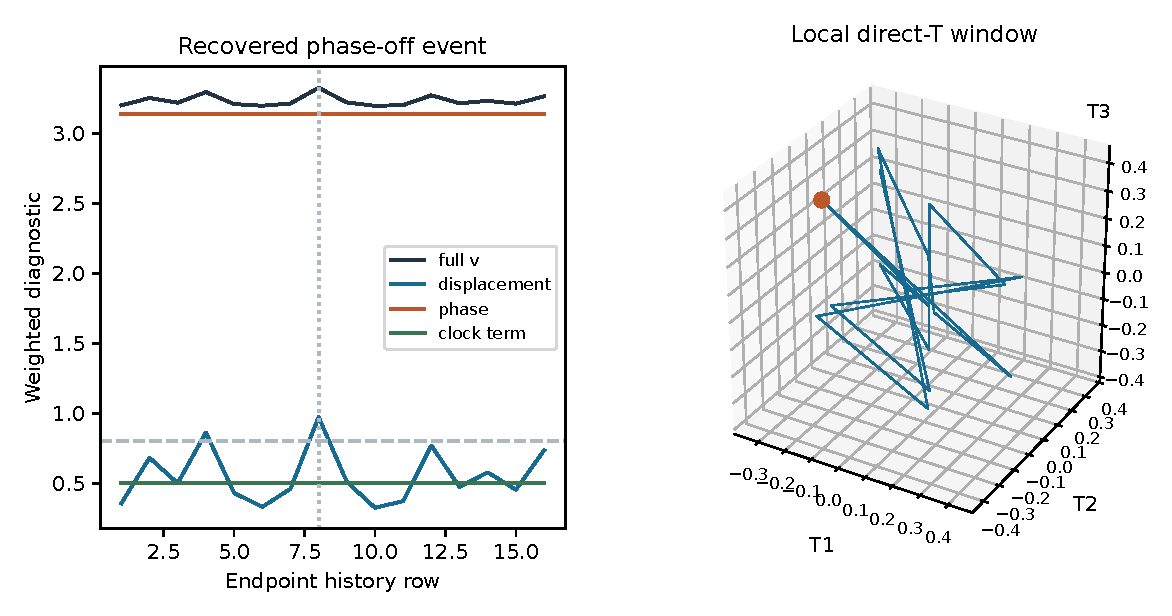
\includegraphics[width=1\linewidth,height=\textheight,keepaspectratio,alt={A finite phase-off event, centered on endpoint row 8 of the subcritical history. The left panel displays the weighted components and their quadratic combination. The right panel shows the local direct-T path.}]{figures/08_spike_window.pdf}
\caption{A finite phase-off event, centered on endpoint row 8 of the subcritical history. The left panel displays the weighted components and their quadratic combination. The right panel shows the local direct-T path.}
\end{figure}

In the critical replay, the early phase term is again close to \(\pi\) for many transitions. At endpoint row 1001, displacement is about \(3.59009\) and the total statistic about \(4.79670\). By row 1276 the displacement is approximately \(3.79\times10^{18}\); by row 1277 it is about \(3.00\times10^{55}\). The macro is bounded by (8) and the staged saturation/envelope, so the enormous total coordinates in this portion require the chiral contribution. This is a component-based diagnosis, not a physical energy interpretation.

The norm computation first overflows at endpoint row 1278 even though the Z coordinates at that row are still finite. Z and \(J\) first become nonfinite at stored row 1279. A nonfinite norm is not equivalent to an already nonfinite input coordinate; sums of squares can overflow earlier. These distinctions are retained in the result files and the shaded failure region of Figure 9. The proof-level cone identity is not falsified by arithmetic that has left its finite domain.

The preserved runs establish phase, clock and displacement mechanisms, and the critical tail establishes chiral growth followed by numerical failure. They do not establish that a particular finite event was caused by exact or near blend cancellation. That mechanism is proved possible by Section 9 and must be diagnosed from component data before attributing it to a run. Event classification in this spike tool does not inject a new dynamical event into \(\Omega\).

\section{15. Reproduction of the preserved runs}\label{reproduction-of-the-preserved-runs}

\subsection{15.1 Settings and initializer}\label{settings-and-initializer}

Both saved configurations use seed 2158500047, 2000 stored rows, \texttt{dt} \(=0.02776\), \(\epsilon=0.0005\), zero forcing and zero complex noise. The seed is used to draw three real and three imaginary standard-normal components; the complex vector is divided by its norm plus \(10^{-12}\). The recovered phase setting is zero. The actual source-selected coefficient triplet is

\paperdisplay[32]{k=(1,\ 1.2208964704604097,\ 6.35310346037241).}

The saved label for a coefficient setting is not substituted for this effective source triplet. The two values of \(g\) are \(0.664\) (subcritical label) and \(0.667\) (critical label). These names identify the preserved experiment; this paper does not establish a global critical-coupling theorem.

{\def\LTcaptype{none} % do not increment counter
\begin{longtable}[]{@{}
  >{\raggedright\arraybackslash}p{(\linewidth - 4\tabcolsep) * \real{0.4800}}
  >{\raggedright\arraybackslash}p{(\linewidth - 4\tabcolsep) * \real{0.2000}}
  >{\raggedright\arraybackslash}p{(\linewidth - 4\tabcolsep) * \real{0.3200}}@{}}
\toprule\noalign{}
\begin{minipage}[b]{\linewidth}\raggedright
Result, zero-based row convention
\end{minipage} & \begin{minipage}[b]{\linewidth}\raggedright
Subcritical
\end{minipage} & \begin{minipage}[b]{\linewidth}\raggedright
Critical
\end{minipage} \\
\midrule\noalign{}
\endhead
\bottomrule\noalign{}
\endlastfoot
Coupling \(g\) & 0.664 & 0.667 \\
Recovered \(\lambda_{\mathrm{phase}}\) & 0 & 0 \\
Saved Z coordinates equal to replay & Yes, all rows & Yes, including nonfinite positions \\
Saved full statistic equal to replay & Yes & Yes, including nonfinite positions \\
Saved \(J\) equal to replay & Yes & Yes, including nonfinite positions \\
Finite events \(v\ge0.8\) & 26 & 1277 \\
First nonfinite Z row & None & 1279 \\
First nonfinite statistic endpoint row & None & 1278 \\
First nonfinite \(J\) row & None & 1279 \\
\end{longtable}
}

The comparison uses exact array equality after parsing the saved decimal CSV fields into the present floating-point representation, with corresponding NaNs treated as equal. It is not merely a tolerance comparison of rendered pictures. Equality of NaN placement is a reproducibility statement about the failure pattern, not numerical validation of the tail as a mathematical solution.

\begin{figure}
\centering
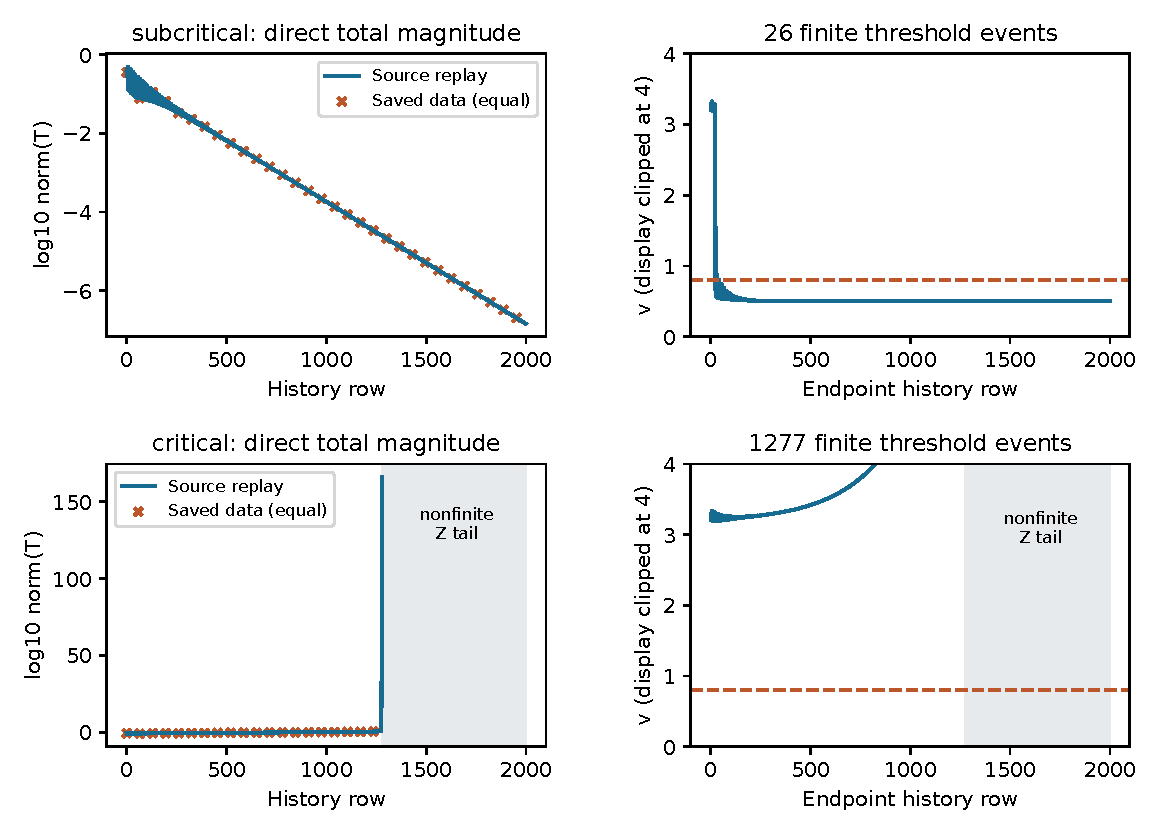
\includegraphics[width=0.94\linewidth,height=\textheight,keepaspectratio,alt={Saved and newly replayed data coincide. The critical statistic panel clips the display at four to expose early behavior; stored arrays are not clipped. Shading starts at the first nonfinite Z row, 1279. Its norm/statistic failure begins one transition earlier.}]{figures/09_preserved_reproduction.pdf}
\caption{Saved and newly replayed data coincide. The critical statistic panel clips the display at four to expose early behavior; stored arrays are not clipped. Shading starts at the first nonfinite Z row, 1279. Its norm/statistic failure begins one transition earlier.}
\end{figure}

\subsection{15.2 What was reused and what was rerun}\label{what-was-reused-and-what-was-rerun}

The earlier verification {[}R{]} tested both the current default phase strength and the phase-off hypothesis. The default produced different saved-run behavior: 27 and 1244 finite threshold events, respectively, and a critical Z failure beginning at row 1246. This contrast demonstrates that silently retaining the current phase default does not reproduce the saved series. It is not a proof that zero is the only possible effective parameterization among all historical programs.

The new Paper E pass reruns only the two recovered configurations, a 300-row viewer baseline and its EMA counterpart, supplying frozen arrays for figures. It does not rerun the earlier 23-configuration parameter study. The original clipped-window checks, involving 1026 and 64827 window rows, are reused from the accepted result record. The original saved packages, summaries and plots remain preserved.

Exact original source-commit and environment attribution remains unresolved. The newly generated output is labelled re-execution output. The package contains enough compact inputs to repeat the fixed checks without copying the wider archive or installing a historical application. Run identity, scientific review status and preservation status are separate fields; passing a replay does not imply acceptance of Paper E\textquotesingle s complete interpretation.

\section{16. Bounded parameter dependence}\label{bounded-parameter-dependence}

\subsection{16.1 Dependency classification}\label{dependency-classification}

The location of a parameter in the equations is more informative than its historical name. The following classification concerns this core with overrides held fixed and noise disabled.

{\def\LTcaptype{none} % do not increment counter
\begin{longtable}[]{@{}
  >{\raggedright\arraybackslash}p{(\linewidth - 2\tabcolsep) * \real{0.2300}}
  >{\raggedright\arraybackslash}p{(\linewidth - 2\tabcolsep) * \real{0.7700}}@{}}
\toprule\noalign{}
\begin{minipage}[b]{\linewidth}\raggedright
Parameter
\end{minipage} & \begin{minipage}[b]{\linewidth}\raggedright
Direct mathematical entry and scope
\end{minipage} \\
\midrule\noalign{}
\endhead
\bottomrule\noalign{}
\endlastfoot
\(\epsilon\) & On-site cubic increment in (3); changes the complex trajectory \\
\(g\) & Graph-coupling increment in (3); changes the complex trajectory \\
\(k_i\) & Channel-specific on-site target coefficients; changes the complex trajectory \\
\(\lambda_{\mathrm{phase}}\) & Additional phase operation (4); can affect subsequent magnitudes indirectly \\
\(\ell\) & Phase of scalar readout; changes macro geometry, not this complex recurrence \\
\(\lambda_{vp}\) & Scalar amplitude multiplier; changes macro readout \\
\(\gamma\) & Staged time-envelope rate; absent from H\textquotesingle s scalar formula \\
\(\alpha,\beta\) & Readout blending weights; change T without changing \(\Omega\) \\
\texttt{dt} & Historical time increment and staged envelope at a fixed row; no factor in (3)-(4) \\
Initial-state seed & Selects initial \(\Omega\) in the specified harness; runner metadata alone is not stochastic seeding \\
\end{longtable}
}

Even though phase synchronization preserves each magnitude in the current step, it changes relative phases entering later graph coupling. It can therefore affect later magnitudes. Conversely, changing a Z readout coefficient does not alter \(\Omega\) in this core. Distinguishing direct dependency from later indirect effects avoids an incorrect claim that all phase changes are dynamically irrelevant.

\subsection{16.2 Reused finite comparisons}\label{reused-finite-comparisons}

The prior baseline uses seed 42, 300 stored rows, \(\epsilon=0.05\), \(g=0.2\), \(\lambda_{\mathrm{phase}}=0.001\), \texttt{dt} \(=0.05\), and the soft coefficient triplet \((1,1.104941840306724,2.52053634379122)\). Its initialization multiplies the random complex draw by \(0.1\) before normalizing by its norm plus \(10^{-12}\), following the viewer setup. This is distinct from the simpler diagnostic wrapper\textquotesingle s small unnormalized seed-zero initializer. ``Default'' without identifying the calling script is consequently ambiguous.

The baseline peak norms from {[}R{]} are approximately \(0.236569\) for M, \(0.126145\) for C and \(0.258789\) for T. The final C norm is about \(1.39\times10^{-17}\), while final T is about \(7.17\times10^{-5}\). These are finite-run results, not a theorem that all chiral trajectories decay.

The bounded one-at-a-time comparisons found peak T near \(0.25660\) and \(0.26098\) for \(\epsilon=0.045,0.055\), and near \(0.27563\) and \(0.24314\) for \(g=0.18,0.22\). Changing the third coefficient by factors \(0.9\) and \(1.1\) gave peaks near \(0.25696\) and \(0.26062\). Phase strengths zero and \(0.002\) changed the recorded vector history relative to the baseline by a maximum norm difference of approximately \(2.20\times10^{-4}\). Seed 43 changed it by approximately \(0.0862\). These measured comparisons are local to the specified run and initial-state construction.

Readout-only changes preserved the complex arrays bit-for-bit in that bounded evidence. Doubling \texttt{dt} to \(0.1\) changed T by a maximum of approximately \(0.10612\) while leaving \(\Omega\) unchanged. Changing the lock to \(0.344\) produced about \(0.07338\) maximum difference. Increasing \(\lambda_{vp}\) by twenty percent produced about \(0.04731\). Setting \(\gamma=0\) raised the peak T to about \(0.44492\) and retained much stronger late clock motion. Pure chiral weighting \(\alpha=0\) gave peak \(0.06307\) with the default \(\beta=0.5\); pure macro weighting \(\beta=0\) gave \(0.23657\); doubling \(\beta\) to one gave approximately \(0.30499\).

These observations agree with the dependency structure and make the display mechanisms concrete. They are not a parameter phase diagram, stability boundary or fitting exercise. No new sweep is needed to establish which symbols appear in (2)-(4). Figure generation uses the frozen finite arrays and does not search for a desired geometric shape.

\section{17. Exact one-step intensity and amplitude budget}\label{exact-one-step-intensity-and-amplitude-budget}

\subsection{17.1 Separation of the three contributions}\label{separation-of-the-three-contributions}

Let \(s_i=|\Omega_i|^2\) and \(I=\|\Omega\|^2=\sum_i s_i\). For the unforced pre-synchronization update define

\paperdisplay[33]{D_i=\epsilon(k_i-s_i)\Omega_i+g(L_3\Omega)_i,
\qquad V=\Omega+D.}

Use the Hermitian inner product \(\langle u,v\rangle=\sum_i\bar u_i v_i\) and real parameters. The complete three-node graph obeys

\paperdisplay[34]{\langle\Omega,L_3\Omega\rangle
=-\sum_{i<j}|\Omega_i-\Omega_j|^2.}

To verify the sign, expand each pair distance as \(|\Omega_i|^2+|\Omega_j|^2-2\Re(\bar\Omega_i\Omega_j)\). Each squared magnitude occurs twice. The negative sum is exactly the diagonal \(-2\) and off-diagonal \(+1\) quadratic form of \(L_3\). The conventional positive graph Laplacian is \(-L_3\) {[}SG{]}.

\textbf{Theorem 11 (exact finite-step intensity budget).} Under these hypotheses,

\paperdisplay[35]{\|V\|^2-I
=2\epsilon\sum_i(k_i s_i-s_i^2)
-2g\sum_{i<j}|\Omega_i-\Omega_j|^2+\|D\|^2.}

\textbf{Proof.} The exact norm expansion is \(\|\Omega+D\|^2-\|\Omega\|^2=2\Re\langle\Omega,D\rangle+\|D\|^2\). The on-site part of the inner product is \(\epsilon\sum_i(k_i-s_i)s_i\). Equation (34) evaluates the coupling part. Multiplying both by two yields (35). No small-step approximation has been used. \(\square\)

The remainder is nonnegative as a whole, even though its expanded cross term may have either sign:

\paperdisplay[36]{\begin{aligned}
\|D\|^2={}&\epsilon^2\sum_i s_i(k_i-s_i)^2+g^2\|L_3\Omega\|^2\\
&+2\epsilon g\Re\sum_i(k_i-s_i)\bar\Omega_i(L_3\Omega)_i.
\end{aligned}}

For \(\epsilon,g\ge0\), graph coupling has a nonpositive first-order contribution to intensity; the on-site term can increase or decrease it depending on the state. The finite-step remainder may outweigh both. A statement about the sign of the first-order terms alone is therefore insufficient to prove monotonic intensity.

\subsection{17.2 Forcing, phase synchronization and limitations}\label{forcing-phase-synchronization-and-limitations}

With deterministic forcing \(\delta\), replace the remainder by \(\|D+\delta\|^2\) and add \(2\Re\langle\Omega,\delta\rangle\) to the right side of (35). This includes the exact forcing cross terms rather than treating \(\delta\) as a physical work term. In exact arithmetic, the separate phase operation preserves \(\|V\|^2\), so the same intensity budget also applies after noiseless synchronization. Optional subsequent noise changes it again. Floating-point reconstruction introduces its usual rounding effects; the identity is an algebraic statement about the defined map.

At a balanced real state with all components equal to two, equal \(k_i=1\), \(\epsilon=1\) and no forcing, coupling vanishes. Each component becomes \(2+2(1-4)=-4\). Intensity rises from 12 to 48. Equation (35) splits this as an on-site contribution \(-72\) and a remainder \(108\), giving \(+36\). This explicit example demonstrates amplitude overshoot even though the on-site first-order contribution is negative. It does not rely on numerical overflow or on the chiral term, which is zero for these real states.

The statistic \(I\) is a channel-amplitude norm. This budget does not turn it, \(V\) or the displayed Z coordinates into a calibrated physical energy. It does supply a precise mechanism by which the discrete state can grow strongly, and hence can permit large quadratic readouts when the real and imaginary vectors span nonzero area.

\section{18. Relation to the existing potential}\label{relation-to-the-existing-potential}

The previously identified real potential is

\paperdisplay[37]{\mathcal V(\Omega)=\epsilon\sum_i\left(\frac{|\Omega_i|^4}{4}
-\frac{k_i|\Omega_i|^2}{2}\right)
+\frac g2\sum_{i<j}|\Omega_i-\Omega_j|^2.}

We use \(\mathcal V\) to distinguish this scalar from the pre-synchronization state \(V\) in (3). The gradient is taken in the six real coordinates \((x_1,x_2,x_3,y_1,y_2,y_3)\) with the ordinary Euclidean metric. No ambiguous complex-gradient convention is needed.

\textbf{Proposition 12 (real gradient increment).} With zero forcing, the pre-synchronization increment satisfies \(D=-\nabla_{\mathbb R^6}\mathcal V\), identifying a complex vector with its real and imaginary parts.

\textbf{Proof.} Since \(s_i=x_i^2+y_i^2\), differentiation of the on-site summand gives \(\epsilon(s_i-k_i)x_i\) in the \(x_i\) direction and \(\epsilon(s_i-k_i)y_i\) in the \(y_i\) direction. Differentiation of the graph term gives \(g\sum_{j\ne i}(x_i-x_j)=-g(L_3x)_i\), and similarly for \(y\). Negating these derivatives gives exactly (33). \(\square\)

\textbf{This gradient-form increment does not imply that the finite update decreases the potential.} The update has a unit step in the real-coordinate gradient convention just specified. There is no state-independent small-step guarantee asserted here. In the balanced example of Section 17, coupling remains zero, and each on-site potential changes from \(4-2=2\) to \(64-8=56\). Thus

\paperdisplay[38]{\mathcal V(2,2,2)=6,\qquad \mathcal V(-4,-4,-4)=168.}

Both the intensity and the potential increase despite the exact negative-gradient increment. A differential gradient flow would have another monotonicity argument, but replacing the inspected finite map by that flow would change the model. The parameter \texttt{dt} in the historical time counter supplies no missing gradient-step factor.

Phase synchronization is an additional operation after the pre-synchronization state has been formed. It preserves all \(s_i\) and hence the on-site part of (37), but it may change pairwise distances and the graph part. It is not established here as a descent step for the same potential. Forcing and noise are further distinct terms. Consequently no universal decrease theorem for the full historical step follows from Proposition 12.

Finally, the source does not identify \(\mathcal V\) with historical ``Z energy.'' The potential is a real scalar on complex channel state space; \(T\) is a three-component readout with an explicit clock and, in K, an external envelope. Conflating these objects would obscure both the exact recurrence and the exact readout geometry. The potential is useful for understanding the increment, while the one-step identity is useful for understanding finite overshoot.

\section{19. Staged envelope and committed EMA}\label{staged-envelope-and-committed-ema}

\subsection{19.1 Two preserved scalar laws}\label{two-preserved-scalar-laws}

The source versions agree on how \(M,C,T\) are formed from their inputs but disagree on the scalar height:

\paperdisplay[39]{\begin{aligned}
\text{K:}\quad z_n&=\lambda_{vp}\rho_n\cos\bigl(3(\theta_n-\ell)\bigr)e^{-\gamma t_n},\\
\text{H:}\quad m_n&=a m_{n-1}+(1-a)j_n,\quad a=0.99,
\quad j_n=\frac{J_n}{1+|J_n|},\\
z_n&=\lambda_{vp}\rho_n\cos\bigl(3(\theta_n-\ell)\bigr)+m_n.
\end{aligned}}

Here the H index \(n\) refers to recomputed states, after updating the memory from the current committed \(\Omega\). Initial stored row zero still follows the constructor convention. The unused \(\gamma\) parameter in H must not be read as a hidden envelope in its scalar formula.

\textbf{Proposition 13 (bounded EMA memory).} If \(|m_0|\le1\) and all \(J_n\) are finite, then \(|m_n|\le1\). More explicitly,

\paperdisplay[40]{m_n=a^n m_0+(1-a)\sum_{j=1}^n a^{n-j}j_j.}

\textbf{Proof.} Repeated substitution proves (40), or induction verifies it directly. Every weight is nonnegative and their sum is \(a^n+(1-a)\sum_{j=1}^n a^{n-j}=1\). Since \(|j_j|<1\) for finite \(J_j\), the expression is a convex combination of values in \([-1,1]\). This proves the stated bound and, after at least one finite input, a strict interior value unless an excluded limiting forcing is used. \(\square\)

This boundedness does not state that the memory decays to zero. Constant nonzero normalized forcing drives it toward that forcing. Nor does it bound the entire blended vector independently of \(\kappa\), because the same chiral term remains present.

\subsection{19.2 Extrema, signs and long-time behavior}\label{extrema-signs-and-long-time-behavior}

Freeze the current \(\rho\) and memory offset, and let \(A_0=\lambda_{vp}\rho\). Then the H angular function is \(A_0\cos(3(\theta-\ell))+m\). For \(A_0\ne0\) it retains six critical angles, since differentiating removes the constant offset. Its two extremal levels are \(m+|A_0|\) and \(m-|A_0|\). Opposite signs occur exactly when \(|m|<|A_0|\); equality makes one extremal level zero, and \(|m|>|A_0|\) makes all heights have the same sign. If \(A_0=0\), the frozen scalar is constant.

The offset preserves the cone identity because the same scalar still multiplies all three macro factors. It generally destroys the half-turn height reversal and the three vertical extremum pairs of the pure harmonic. A claim about six angular extrema can therefore remain true while a claim about three upper and three lower points becomes false. Along an actual run, both \(\rho\) and memory change, adding another reason not to transfer the frozen pairing theorem to an EMA trajectory.

\begin{figure}
\centering
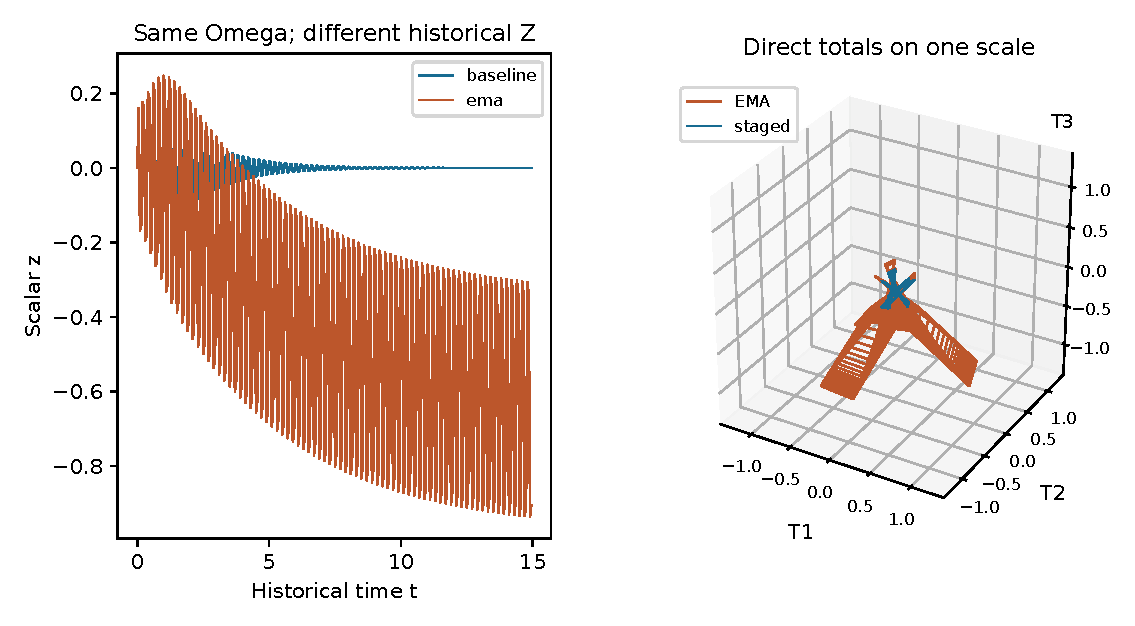
\includegraphics[width=1\linewidth,height=\textheight,keepaspectratio,alt={Identical complex-state evolution with two historical scalar laws. The staged envelope and committed EMA produce different scalar histories and direct totals. The two direct paths use one common raw coordinate scale.}]{figures/10_staged_ema.pdf}
\caption{Identical complex-state evolution with two historical scalar laws. The staged envelope and committed EMA produce different scalar histories and direct totals. The two direct paths use one common raw coordinate scale.}
\end{figure}

The baseline and EMA figure replays use the same complex update and initial state. Their \(\Omega\) histories agree, while the EMA total\textquotesingle s final norm in the accepted finite comparison is about \(1.279\), compared with roughly \(7.17\times10^{-5}\) for the staged total. These numbers demonstrate the particular finite runs, not an asymptotic theorem about every trajectory. Under \(\gamma>0\) and \(t\to+\infty\), the staged macro envelope tends to zero because \(\rho\le1\). Its chiral term still has no imposed decay envelope and need not decay. H has no corresponding exponential factor at all. The versions must therefore retain separate long-time statements.

\section{20. The open six-gap interface}\label{the-open-six-gap-interface}

Four facts now coexist without contradiction. The scalar\textquotesingle s six-extrema theorem is proved. The source-defined direct Z mechanism is recovered. The author recalls a Z-vector or torus curve moving through or between an upper/lower gap structure. Paper D supplies an exact reference-scaffold construction. What is absent from the bounded evidence is the rule attaching the source trajectory to six three-dimensional scaffold openings.

Paper D\textquotesingle s clarified planar construction has three selected edges alternating with three connectors, an explicit positive-length domain, an equilateral support triangle and three corner cells. It distinguishes that reference concept from the separately specified welded realization. Those geometric results do not by themselves determine where a source vector lives in a three-dimensional opening arrangement. The numbers six, three and twelve appearing in the different constructions are not a substitute for a map.

\begin{figure}
\centering
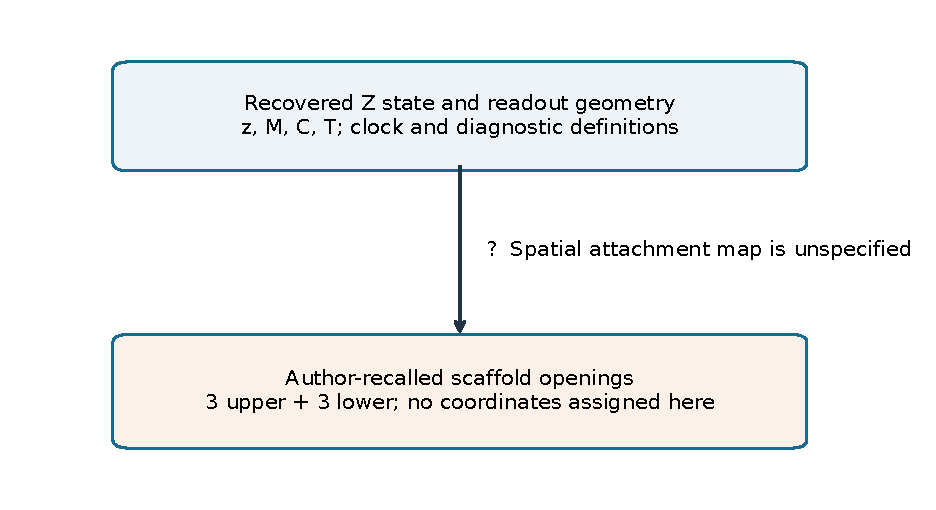
\includegraphics[width=0.9\linewidth,height=\textheight,keepaspectratio,alt={The remaining interface. Boxes denote defined and author-recalled objects, not geometric anchor coordinates. The question mark records the missing spatial registration.}]{figures/11_open_interface.pdf}
\caption{The remaining interface. Boxes denote defined and author-recalled objects, not geometric anchor coordinates. The question mark records the missing spatial registration.}
\end{figure}

The exact missing fact is whether Z was placed directly in a scaffold frame or transformed into independently specified upper and lower gap anchors, together with the transform and the clock-to-gap correspondence. The inspected direct-vector helper only returns stored coordinates; scalar and channel torus helpers use their own formulas; UI ``gap'' variables place controls. None establishes that fact. The missing claim is therefore the \textbf{spatial attachment}, not the existence or definition of Z.

In particular, the sequence (10) cannot be called a recovered gap order. It concerns six extrema of a frozen harmonic, while the default clock does not hit them. A genuine registration might use a continuous interpolation, clock samples, a normalized total direction or another construction, and these choices are mathematically different. Selecting one without evidence would be a new model choice. No such choice is made here.

The author clarification is present-day design evidence, not a recovered old equation. No exact source closing this interface was found during bounded citation preparation; no broad search was launched. This open status permits completion of the present mathematics paper. It does not authorize Z restoration, geometry adoption or a gap-flux rule in the current implementation.

\section{21. Connections to standard mathematics}\label{connections-to-standard-mathematics}

The scalar is a Fourier harmonic on the circle. Its eigenvalue equation is \(f''+9f=0\) at fixed amplitude, and its sampled clock exhibits the elementary consequences of evaluating that harmonic on a finite cyclic grid. This observation explains the six critical angles and the repeated four-value pattern without additional geometric assumptions.

The signed polar projection is a rhodonea {[}Erb{]}, while multiplication by a rotating unit vector yields the Cartesian frequency shifts in (11). The macro cone is a quadratic surface in the direct plotting coordinates. These are compatible descriptions of one defined map: the cone constrains its three-dimensional endpoints, and the rose describes their frozen planar image. They do not make its discrete polyline a smooth embedded manifold.

The chiral observable is the standard oriented area of two real vectors. Its squared magnitude is a two-vector Gram determinant, and the bound follows from an explicit sum of squares {[}VA{]}. Its channel interpretation, rather than an unprovided ambient-vector interpretation, is the connection carried forward from Paper B.

The recurrence uses the negative of the conventional positive Laplacian of the complete three-node graph. The pair-distance identity is the usual graph quadratic form {[}SG{]}, with its sign stated explicitly. Combined with the on-site cubic, it produces a finite discrete map whose exact norm budget includes a quadratic remainder. Gradient-form increments and monotone gradient flows are distinct mathematical objects.

Vector blending, normalization and finite-difference diagnostics supply the remaining tools. The norm identity is bilinear algebra; directional instability near zero follows from differentiating normalization; the full statistic is a weighted Euclidean norm of heterogeneous diagnostic components. These standard connections explain the construction without treating the chosen coordinates or coefficients as calibrated physical quantities.

\section{22. Interpretation limits and evidential scope}\label{interpretation-limits-and-evidential-scope}

Z is a historically named emergent readout, and ``Z energy'' is project terminology. No calibrated physical energy unit, conservation theorem, field stress tensor, gap-flux law or physical particle identification is established in this manuscript. A plotted trajectory is an exact finite sequence of defined readouts when its numerical inputs are finite; a line renderer adds straight connections. An infinite or NaN array entry is a computational failure, not an infinite physical quantity.

These limits do not weaken the positive mathematical results. The source defines an explicit hierarchy of observables. The cone constraint, harmonic decomposition, channel-area laws, sharp bound, blending identities and finite-step budget are exact consequences of those definitions. The source maps and reproduced arrays establish what the inspected historical program computes. The package makes the distinctions testable by preserving the relevant originals and supplying independent algebra checks.

Theorems have deliberately different scopes. Frozen-angle extrema and symmetries require fixed amplitude. The cone identity requires only the macro definition. The channel-area identities require finite complex input and the specified ordered channel coordinates. The cancellation criterion is pointwise and does not certify dynamic attainability. The intensity budget concerns the specified pre-sync map, with phase preservation and forcing qualifications stated separately. The recorded finite runs do not prove global stability or establish a physical critical point.

Source recovery and historical attribution also remain distinct. Exact saved-array reproduction identifies a compatible effective configuration, not the original commit or environment. Existing reports are evidence rather than new independent acceptance. Paper E itself is submitted for GPT\textquotesingle s full scientific review. It does not claim joint acceptance of material beyond prior reviews\textquotesingle{} actual scope.

\section{23. Conclusion}\label{conclusion}

The historical Z system is a mathematically explicit composite readout. A third-harmonic clock-driven macro lies on a double cone and is deformed by a quadratic, orientation-sensitive channel observable. Its frozen extrema, signed visiting order, planar rose projection and symmetry transformations follow from the formulas. The default twelve-sector sampling, changing amplitudes and retained polyline history explain why its displayed arms differ from a smooth ideal curve.

The direct trajectory, scalar cylinder, history torus, channel-torus curves and percentile-scaled overlay are now distinguished at the level of equations and information content. The full spike statistic is separated from directional turning, segment curvature and entropy change. Recovered phase-off settings reproduce the two preserved datasets exactly, while their finite events and numerical failure tail retain separate meanings. The one-step intensity identity and potential counterexample explain why the finite recurrence need not be a monotone descent process.

The staged envelope and the committed EMA remain separate historical variants. The remaining geometric interface is the spatial attachment to six author-recalled scaffold openings. It is not an ambiguity in the recovered definition of Z. This manuscript closes the source-defined mathematics within its stated scope and records that specific attachment as open for later evidence, without supplying a new law or changing the implementation.

\section{References}\label{references}

\textbf{{[}R{]}} Codex, with author/design testimony by Hilmir Frímann Halldórsson. \emph{Historical Z manifold and six-gap reconstruction v0.1}. 23 September 2026. Primary accepted reconstruction for this work order. The unchanged report and verification results are included in the accepted-reconstruction evidence folder; the reference ledger records the exact original path. The report\textquotesingle s source hashes identify the inspected K and H code.

\textbf{{[}B{]}} Hilmir Frímann Halldórsson. \emph{Triadic Chirality and Orientation Geometry}. Paper B, publication revision v0.1.2, 2026. Repository package \texttt{papers/PAPER\_B/publication/v0.1.2/}. Used only for its accepted channel-space area interpretation and related transformation laws. Full publication title and PDF identity are recorded in the reference ledger.

\textbf{{[}D{]}} Hilmir Frímann Halldórsson. \emph{Tri-Octagon Reference-Scaffold Geometry: Exact Construction of an Alternating Hexagonal Core}. Paper D, v0.1.1, 23 September 2026. Repository package \texttt{papers/PAPER\_D/v0.1.1/}. Used only for the clarified reference-scaffold geometry and the preserved distinction between known construction and unresolved Z attachment.

\textbf{{[}Erb{]}} Wolfgang Erb. \emph{Rhodonea curves as sampling trajectories for spectral interpolation on the unit disk}. arXiv:1812.00437v1, 2 December 2018. \href{https://arxiv.org/abs/1812.00437}{arXiv record}. Example 3(iv), p. 10, supplies the odd-frequency petal convention. Model-specific derivations in this manuscript do not depend on the paper\textquotesingle s interpolation results.

\textbf{{[}VA{]}} Harvey Mudd College Mathematics. \emph{Elementary Vector Analysis}, Calculus Online Tutorials, undated. \href{https://math.hmc.edu/calculus/hmc-mathematics-calculus-online-tutorials/multivariable-calculus/elementary-vector-analysis/}{Institutional tutorial}. Cross-product section: Lagrange identity and parallelogram area. Accessed 23 September 2026. The specific channel identity and equality case are independently proved here.

\textbf{{[}SG{]}} Daniel A. Spielman. \emph{Spectral Graph Theory, Lecture 2: The Laplacian}. Yale University, 4 September 2009. \href{https://www.cs.yale.edu/homes/spielman/561/2009/lect02-09.pdf}{Lecture notes}. Page 2, equation (2.2), gives the standard positive-Laplacian quadratic form. Our source matrix has the opposite sign.

\end{document}
